%%%%%%%%%%%%%%%%%%%%%%%%%%%%%%%%%%%%%%%%%
% The Legrand Orange Book
% LaTeX Template
% Version 1.4 (12/4/14)
%
% This template has been downloaded from:
% http://www.LaTeXTemplates.com
%
% Original author:
% Mathias Legrand (legrand.mathias@gmail.com)
%
% License:
% CC BY-NC-SA 3.0 (http://creativecommons.org/licenses/by-nc-sa/3.0/)
%
% Compiling this template:
% This template uses biber for its bibliography and makeindex for its index.
% When you first open the template, compile it from the command line with the 
% commands below to make sure your LaTeX distribution is configured correctly:
%
% 1) pdflatex oqhbt
% 1a) pdflatex -shell-escape oqhbt
% 2) makeindex oqhbt.idx -s StyleInd.ist
% 3) biber oqhbt
% 4  makeglossaries oqhbt
% 4) pdflatex oqhbt x 2
%
% After this, when you wish to update the bibliography/index use the appropriate
% command above and make sure to compile with pdflatex several times 
% afterwards to propagate your changes to the document.
%
% This template also uses a number of packages which may need to be
% updated to the newest versions for the template to compile. It is strongly
% recommended you update your LaTeX distribution if you have any
% compilation errors.
%
% Important note:
% Chapter heading images should have a 2:1 width:height ratio,
% e.g. 920px width and 460px height.
%
%%%%%%%%%%%%%%%%%%%%%%%%%%%%%%%%%%%%%%%%%

%----------------------------------------------------------------------------------------
%	PACKAGES AND OTHER DOCUMENT CONFIGURATIONS
%----------------------------------------------------------------------------------------

\documentclass[11pt,fleqn]{book} % Default font size and left-justified equations

\usepackage[top=3cm,bottom=3cm,left=3.2cm,right=3.2cm,headsep=10pt,a4paper]{geometry} % Page margins

\usepackage{xcolor} % Required for specifying colors by name
\definecolor{ocre}{RGB}{243,102,25} % Define the orange color used for highlighting throughout the book

% Font Settings
\usepackage{avant} % Use the Avantgarde font for headings
%\usepackage{times} % Use the Times font for headings
\usepackage{mathptmx} % Use the Adobe Times Roman as the default text font together with math symbols from the Sym­bol, Chancery and Com­puter Modern fonts

\usepackage{microtype} % Slightly tweak font spacing for aesthetics
\usepackage[utf8]{inputenc} % Required for including letters with accents
\usepackage[T1]{fontenc} % Use 8-bit encoding that has 256 glyphs

% Bibliography
\usepackage{csquotes}
\usepackage[style=alphabetic,
            sorting=nyt,
            sortcites=true,
            natbib=true,
            style=authoryear,
            maxcitenames=2,
            maxbibnames=100,
            autopunct=true,
            babel=hyphen,
            hyperref=true,
            doi=true,
            abbreviate=false,
            backref=true,
            backend=biber]{biblatex}
\addbibresource{./Bibliography/hazard.bib} % BibTeX bibliography file
\defbibheading{bibempty}{}

% Figure caption settings
\usepackage[textfont=it,margin=10pt,font=small,labelfont=bf,labelsep=endash]{caption}

% Table - colors from 
\usepackage{verbatim}
\usepackage{color, colortbl}
\definecolor{almond}{rgb}{0.94, 0.87, 0.8}
\definecolor{ashgrey}{rgb}{0.7, 0.75, 0.71}
\definecolor{anti-flashwhite}{rgb}{0.95, 0.95, 0.96}
\definecolor{anti-flashwhite}{rgb}{0.95, 0.95, 0.96}
\definecolor{airforceblue}{rgb}{0.36, 0.54, 0.66}

% Index
\usepackage{calc} % For simpler calculation - used for spacing the index letter headings correctly
\usepackage{makeidx} % Required to make an index
\makeindex % Tells LaTeX to create the files required for indexing

\usepackage{todonotes}
\usepackage{geometry}
\usepackage{marginnote}

%
% Package to create a glossary - It must be uploaded after hyperref
% to produce the glossary: makeglossaries OQB
\usepackage[acronym,nonumberlist,style=altlist]{glossaries}
\glstoctrue
\makeglossaries

% package for bold symbols
\usepackage{bm}

% for better looking tables
\usepackage{ctable}
%
% For embedding code
\usepackage{listings}
\lstset{language=Python}

%----------------------------------------------------------------------------------------
% Trees
%\usepackage[pdf]{pstricks}
%\usepackage{auto-pst-pdf}
%\usepackage{pst-tree}
%
%-------------------------------------------------------------------------------
% Insert the commands.tex file which contains the majority of the structure 
% behind the template
%----------------------------------------------------------------------------------------
%	VARIOUS REQUIRED PACKAGES
%----------------------------------------------------------------------------------------

\usepackage{titlesec} % Allows customization of titles

\usepackage{graphicx} % Required for including pictures
\graphicspath{{Pictures/}} % Specifies the directory where pictures are stored

\usepackage{tikz} % Required for drawing custom shapes

\usepackage[english]{babel} % English language/hyphenation

\usepackage{enumitem} % Customize lists
\setlist{nolistsep} % Reduce spacing between bullet points and numbered lists

\usepackage{booktabs} % Required for nicer horizontal rules in tables

\usepackage{eso-pic} % Required for specifying an image background in the title page

%----------------------------------------------------------------------------------------
%	MAIN TABLE OF CONTENTS
%----------------------------------------------------------------------------------------

\usepackage{titletoc} % Required for manipulating the table of contents

\contentsmargin{0cm} % Removes the default margin
% Chapter text styling
\titlecontents{chapter}[1.25cm] % Indentation
{\addvspace{15pt}\large\sffamily\bfseries} % Spacing and font options for chapters
{\color{ocre!60}\contentslabel[\Large\thecontentslabel]{1.25cm}\color{ocre}} % Chapter number
{}  
{\color{ocre!60}\normalsize\sffamily\bfseries\;\titlerule*[.5pc]{.}\;\thecontentspage} % Page number
% Section text styling
\titlecontents{section}[1.25cm] % Indentation
{\addvspace{5pt}\sffamily\bfseries} % Spacing and font options for sections
{\contentslabel[\thecontentslabel]{1.25cm}} % Section number
{}
{\sffamily\hfill\color{black}\thecontentspage} % Page number
[]
% Subsection text styling
\titlecontents{subsection}[1.25cm] % Indentation
{\addvspace{1pt}\sffamily\small} % Spacing and font options for subsections
{\contentslabel[\thecontentslabel]{1.25cm}} % Subsection number
{}
{\sffamily\;\titlerule*[.5pc]{.}\;\thecontentspage} % Page number
[] 

%----------------------------------------------------------------------------------------
%	MINI TABLE OF CONTENTS IN CHAPTER HEADS
%----------------------------------------------------------------------------------------

% Section text styling
\titlecontents{lsection}[0em] % Indendating
{\footnotesize\sffamily} % Font settings
{}
{}
{}

% Subsection text styling
\titlecontents{lsubsection}[.5em] % Indentation
{\normalfont\footnotesize\sffamily} % Font settings
{}
{}
{}
 
%----------------------------------------------------------------------------------------
%	PAGE HEADERS
%----------------------------------------------------------------------------------------

\usepackage{fancyhdr} % Required for header and footer configuration

\pagestyle{fancy}
\renewcommand{\chaptermark}[1]{\markboth{\sffamily\normalsize\bfseries\chaptername\ \thechapter.\ #1}{}} % Chapter text font settings
\renewcommand{\sectionmark}[1]{\markright{\sffamily\normalsize\thesection\hspace{5pt}#1}{}} % Section text font settings
\fancyhf{} \fancyhead[LE,RO]{\sffamily\normalsize\thepage} % Font setting for the page number in the header
\fancyhead[LO]{\rightmark} % Print the nearest section name on the left side of odd pages
\fancyhead[RE]{\leftmark} % Print the current chapter name on the right side of even pages
\renewcommand{\headrulewidth}{0.5pt} % Width of the rule under the header
\addtolength{\headheight}{2.5pt} % Increase the spacing around the header slightly
\renewcommand{\footrulewidth}{0pt} % Removes the rule in the footer
\fancypagestyle{plain}{\fancyhead{}\renewcommand{\headrulewidth}{0pt}} % Style for when a plain pagestyle is specified

% Removes the header from odd empty pages at the end of chapters
\makeatletter
\renewcommand{\cleardoublepage}{
\clearpage\ifodd\c@page\else
\hbox{}
\vspace*{\fill}
\thispagestyle{empty}
\newpage
\fi}

%----------------------------------------------------------------------------------------
%	THEOREM STYLES
%----------------------------------------------------------------------------------------

\usepackage{amsmath,amsfonts,amssymb,amsthm} % For math equations, theorems, symbols, etc

\newcommand{\intoo}[2]{\mathopen{]}#1\,;#2\mathclose{[}}
\newcommand{\ud}{\mathop{\mathrm{{}d}}\mathopen{}}
\newcommand{\intff}[2]{\mathopen{[}#1\,;#2\mathclose{]}}
\newtheorem{notation}{Notation}[chapter]

%%%%%%%%%%%%%%%%%%%%%%%%%%%%%%%%%%%%%%%%%%%%%%%%%%%%%%%%%%%%%%%%%%%%%%%%%%%
%%%%%%%%%%%%%%%%%%%% dedicated to boxed/framed environements %%%%%%%%%%%%%%
%%%%%%%%%%%%%%%%%%%%%%%%%%%%%%%%%%%%%%%%%%%%%%%%%%%%%%%%%%%%%%%%%%%%%%%%%%%
\newtheoremstyle{ocrenumbox}% % Theorem style name
{0pt}% Space above
{0pt}% Space below
{\normalfont}% % Body font
{}% Indent amount
{\small\bf\sffamily\color{ocre}}% % Theorem head font
{\;}% Punctuation after theorem head
{0.25em}% Space after theorem head
{\small\sffamily\color{ocre}\thmname{#1}\nobreakspace\thmnumber{\@ifnotempty{#1}{}\@upn{#2}}% Theorem text (e.g. Theorem 2.1)
\thmnote{\nobreakspace\the\thm@notefont\sffamily\bfseries\color{black}---\nobreakspace#3.}} % Optional theorem note
\renewcommand{\qedsymbol}{$\blacksquare$}% Optional qed square

\newtheoremstyle{blacknumex}% Theorem style name
{5pt}% Space above
{5pt}% Space below
{\normalfont}% Body font
{} % Indent amount
{\small\bf\sffamily}% Theorem head font
{\;}% Punctuation after theorem head
{0.25em}% Space after theorem head
{\small\sffamily{\tiny\ensuremath{\blacksquare}}\nobreakspace\thmname{#1}\nobreakspace\thmnumber{\@ifnotempty{#1}{}\@upn{#2}}% Theorem text (e.g. Theorem 2.1)
\thmnote{\nobreakspace\the\thm@notefont\sffamily\bfseries---\nobreakspace#3.}}% Optional theorem note

\newtheoremstyle{blacknumbox} % Theorem style name
{0pt}% Space above
{0pt}% Space below
{\normalfont}% Body font
{}% Indent amount
{\small\bf\sffamily}% Theorem head font
{\;}% Punctuation after theorem head
{0.25em}% Space after theorem head
{\small\sffamily\thmname{#1}\nobreakspace\thmnumber{\@ifnotempty{#1}{}\@upn{#2}}% Theorem text (e.g. Theorem 2.1)
\thmnote{\nobreakspace\the\thm@notefont\sffamily\bfseries---\nobreakspace#3.}}% Optional theorem note

%%%%%%%%%%%%%%%%%%%%%%%%%%%%%%%%%%%%%%%%%%%%%%%%%%%%%%%%%%%%%%%%%%%%%%%%%%%
%%%%%%%%%%%%% dedicated to non-boxed/non-framed environements %%%%%%%%%%%%%
%%%%%%%%%%%%%%%%%%%%%%%%%%%%%%%%%%%%%%%%%%%%%%%%%%%%%%%%%%%%%%%%%%%%%%%%%%%
\newtheoremstyle{ocrenum}% % Theorem style name
{5pt}% Space above
{5pt}% Space below
{\normalfont}% % Body font
{}% Indent amount
{\small\bf\sffamily\color{ocre}}% % Theorem head font
{\;}% Punctuation after theorem head
{0.25em}% Space after theorem head
{\small\sffamily\color{ocre}\thmname{#1}\nobreakspace\thmnumber{\@ifnotempty{#1}{}\@upn{#2}}% Theorem text (e.g. Theorem 2.1)
\thmnote{\nobreakspace\the\thm@notefont\sffamily\bfseries\color{black}---\nobreakspace#3.}} % Optional theorem note
\renewcommand{\qedsymbol}{$\blacksquare$}% Optional qed square
\makeatother

% Defines the theorem text style for each type of theorem to one of the three styles above
\newcounter{dummy} 
\numberwithin{dummy}{section}
\theoremstyle{ocrenumbox}
\newtheorem{theoremeT}[dummy]{Theorem}
\newtheorem{problem}{Problem}[chapter]
\newtheorem{exerciseT}{Exercise}[chapter]
\theoremstyle{blacknumex}
\newtheorem{exampleT}{Example}[chapter]
\theoremstyle{blacknumbox}
\newtheorem{vocabulary}{Vocabulary}[chapter]
\newtheorem{definitionT}{Definition}[section]
\newtheorem{corollaryT}[dummy]{Corollary}
\theoremstyle{ocrenum}
\newtheorem{proposition}[dummy]{Proposition}

%----------------------------------------------------------------------------------------
%	DEFINITION OF COLORED BOXES
%----------------------------------------------------------------------------------------

\RequirePackage[framemethod=default]{mdframed} % Required for creating the theorem, definition, exercise and corollary boxes

% Theorem box
\newmdenv[skipabove=7pt,
skipbelow=7pt,
backgroundcolor=black!5,
linecolor=ocre,
innerleftmargin=5pt,
innerrightmargin=5pt,
innertopmargin=5pt,
leftmargin=0cm,
rightmargin=0cm,
innerbottommargin=5pt]{tBox}

% Exercise box	  
\newmdenv[skipabove=7pt,
skipbelow=7pt,
rightline=false,
leftline=true,
topline=false,
bottomline=false,
backgroundcolor=ocre!10,
linecolor=ocre,
innerleftmargin=5pt,
innerrightmargin=5pt,
innertopmargin=5pt,
innerbottommargin=5pt,
leftmargin=0cm,
rightmargin=0cm,
linewidth=4pt]{eBox}	

% Definition box
\newmdenv[skipabove=7pt,
skipbelow=7pt,
rightline=false,
leftline=true,
topline=false,
bottomline=false,
linecolor=ocre,
innerleftmargin=5pt,
innerrightmargin=5pt,
innertopmargin=0pt,
leftmargin=0cm,
rightmargin=0cm,
linewidth=4pt,
innerbottommargin=0pt]{dBox}	

% Corollary box
\newmdenv[skipabove=7pt,
skipbelow=7pt,
rightline=false,
leftline=true,
topline=false,
bottomline=false,
linecolor=gray,
backgroundcolor=black!5,
innerleftmargin=5pt,
innerrightmargin=5pt,
innertopmargin=5pt,
leftmargin=0cm,
rightmargin=0cm,
linewidth=4pt,
innerbottommargin=5pt]{cBox}

% Creates an environment for each type of theorem and assigns it a theorem text style from the "Theorem Styles" section above and a colored box from above
\newenvironment{theorem}{\begin{tBox}\begin{theoremeT}}{\end{theoremeT}\end{tBox}}
\newenvironment{exercise}{\begin{eBox}\begin{exerciseT}}{\hfill{\color{ocre}\tiny\ensuremath{\blacksquare}}\end{exerciseT}\end{eBox}}				  
\newenvironment{definition}{\begin{dBox}\begin{definitionT}}{\end{definitionT}\end{dBox}}	
\newenvironment{example}{\begin{exampleT}}{\hfill{\tiny\ensuremath{\blacksquare}}\end{exampleT}}		
\newenvironment{corollary}{\begin{cBox}\begin{corollaryT}}{\end{corollaryT}\end{cBox}}	

%----------------------------------------------------------------------------------------
%	REMARK ENVIRONMENT
%----------------------------------------------------------------------------------------

\newenvironment{remark}{\par\vspace{10pt}\small % Vertical white space above the remark and smaller font size
\begin{list}{}{
\leftmargin=35pt % Indentation on the left
\rightmargin=25pt}\item\ignorespaces % Indentation on the right
\makebox[-2.5pt]{\begin{tikzpicture}[overlay]
\node[draw=ocre!60,line width=1pt,circle,fill=ocre!25,font=\sffamily\bfseries,inner sep=2pt,outer sep=0pt] at (-15pt,0pt){\textcolor{ocre}{R}};\end{tikzpicture}} % Orange R in a circle
\advance\baselineskip -1pt}{\end{list}\vskip5pt} % Tighter line spacing and white space after remark

%----------------------------------------------------------------------------------------
%	SECTION NUMBERING IN THE MARGIN
%----------------------------------------------------------------------------------------

\makeatletter
\renewcommand{\@seccntformat}[1]{\llap{\textcolor{ocre}{\csname the#1\endcsname}\hspace{1em}}}                    
\renewcommand{\section}{\@startsection{section}{1}{\z@}
{-4ex \@plus -1ex \@minus -.4ex}
{1ex \@plus.2ex }
{\normalfont\large\sffamily\bfseries}}
\renewcommand{\subsection}{\@startsection {subsection}{2}{\z@}
{-3ex \@plus -0.1ex \@minus -.4ex}
{0.5ex \@plus.2ex }
{\normalfont\sffamily\bfseries}}
\renewcommand{\subsubsection}{\@startsection {subsubsection}{3}{\z@}
{-2ex \@plus -0.1ex \@minus -.2ex}
{.2ex \@plus.2ex }
{\normalfont\small\sffamily\bfseries}}                        
\renewcommand\paragraph{\@startsection{paragraph}{4}{\z@}
{-2ex \@plus-.2ex \@minus .2ex}
{.1ex}
{\normalfont\small\sffamily\bfseries}}

%----------------------------------------------------------------------------------------
%	HYPERLINKS IN THE DOCUMENTS
%----------------------------------------------------------------------------------------

% For an unclear reason, the package should be loaded now and not later
\usepackage{hyperref}
\hypersetup{hidelinks,backref=true,pagebackref=true,hyperindex=true,colorlinks=false,breaklinks=true,urlcolor= ocre,bookmarks=true,bookmarksopen=false,pdftitle={Title},pdfauthor={Author}}

%----------------------------------------------------------------------------------------
%	CHAPTER HEADINGS
%----------------------------------------------------------------------------------------

% The set-up below should be (sadly) manually adapted to the overall margin page
% septup controlled by the geometry package loaded in the main.tex document. It
% is possible to implement below the dimensions used in the goemetry package
% (top,bottom,left,right)... TO BE DONE

\newcommand{\thechapterimage}{}
\newcommand{\chapterimage}[1]{\renewcommand{\thechapterimage}{#1}}

% Numbered chapters with mini tableofcontents
\def\thechapter{\arabic{chapter}}
\def\@makechapterhead#1{
\thispagestyle{empty}
{\centering \normalfont\sffamily
\ifnum \c@secnumdepth >\m@ne
\if@mainmatter
\startcontents
\begin{tikzpicture}[remember picture,overlay]
\node at (current page.north west)
{\begin{tikzpicture}[remember picture,overlay]
\node[anchor=north west,inner sep=0pt] at (0,0) {\includegraphics[width=\paperwidth]{\thechapterimage}};
%%%%%%%%%%%%%%%%%%%%%%%%%%%%%%%%%%%%%%%%%%%%%%%%%%%%%%%%%%%%%%%%%%%%%%%%%%%%%%%%%%%%%
% Commenting the 3 lines below removes the small contents box in the chapter heading
\fill[color=ocre!10!white,opacity=.6] (1cm,0) rectangle (8cm,-7cm);
\node[anchor=north west] at (1.1cm,.35cm) {\parbox[t][8cm][t]{6.5cm}{
    \huge\bfseries\flushleft \printcontents{l}{1}{\setcounter{tocdepth}{2}}}};
\draw[anchor=west] (5cm,-9cm) node [rounded corners=20pt,fill=ocre!10!white,text opacity=1,draw=ocre,draw opacity=1,line width=1.5pt,fill opacity=.6,inner sep=12pt]{\huge\sffamily\bfseries\textcolor{black}{\thechapter. #1\strut\makebox[22cm]{}}};
%%%%%%%%%%%%%%%%%%%%%%%%%%%%%%%%%%%%%%%%%%%%%%%%%%%%%%%%%%%%%%%%%%%%%%%%%%%%%%%%%%%%%
\end{tikzpicture}};
\end{tikzpicture}}
\par\vspace*{230\p@}
\fi
\fi}

% Unnumbered chapters without mini tableofcontents (could be added though) 
\def\@makeschapterhead#1{
\thispagestyle{empty}
{\centering \normalfont\sffamily
\ifnum \c@secnumdepth >\m@ne
\if@mainmatter
\begin{tikzpicture}[remember picture,overlay]
\node at (current page.north west)
{\begin{tikzpicture}[remember picture,overlay]
\node[anchor=north west,inner sep=0pt] at (0,0) {\includegraphics[width=\paperwidth]{\thechapterimage}};
\draw[anchor=west] (5cm,-9cm) node [rounded corners=20pt,fill=ocre!10!white,fill opacity=.6,inner sep=12pt,text opacity=1,draw=ocre,draw opacity=1,line width=1.5pt]{\huge\sffamily\bfseries\textcolor{black}{#1\strut\makebox[22cm]{}}};
\end{tikzpicture}};
\end{tikzpicture}}
\par\vspace*{230\p@}
\fi
\fi
}
\makeatother
 
%
\begin{document}
% - - - - - - - - - - - - - - - - - - - - - - - - - - - - - -  Load the glossary
% OpenQuake Book Glossary 
% To cite a glossary element in a document:
%	\gls{seismicsourcedata}
%	\Gls{seismicsourcedata} - First initial is uppercase
%	\GLS{seismicsourcedata} - All initials are uppercase
%	\glspl{seismicsourcedata} - Plural
% To process the glossary:
% 	makeglossaries oqb

%
% ------- A
\newglossaryentry{areasource}{
	name = area source,
	description={PSHA source typology usually adopted to model distributed 
	seismicity. The rate of occurrence of seismicity is assumed uniform over
	the source area; this produces an hazard pattern consisting of a more or 
	less uniform patch resembling the shape of the polygon smoothed at the 
	borders}
}
%
% ------- B
\newglossaryentry{branch}{
	name = branch,
	plural= branches,
	description={
	The simplest element in a logic tree; it belongs to a 
	\gls{branchset} where it represents one possible option among a finite 
	number of alternatives. A branch is associated with a weight 
	value \citep{scherbaum2011} if the \gls{branchset} represents the 
	epistemic uncertainty on a parameter or a model when the \gls{branchset} 
	is used to specify alternative models (e.g. district \glspl{acr:mfd})
	}
}
\newglossaryentry{branchinglevel}{
	name = branching level,
	description={It indicates the position where a \gls{branchset} or a 
	\gls{branch} is located in a logic tree structure. For example, 
	in \gls{acr:oq} the first branching level of the 
	\gls{seismicsourcelogictree} always contains one or several 
	\glspl{initialseismicsourcemodel}
	}
}
\newglossaryentry{branchset}{
	name = branch set,
	description={The structure describing the epistemic uncertainty on 
	a specific parameter or model included in a logic tree structure. 
	It ensembles a number of \glspl{branch}, each one representing a 
	discrete alternative}
}
%
% ------- C
\newacronym{cpsha}{cPSHA}{Classical PSHA}
\newglossaryentry{configurationfile}{
	name =  configuration file,
	description = {
	Usually the file containing the information necessary to run a calculation
	in OpenQuake
	}
}
\newglossaryentry{complexfaultsource}{
	name = complex fault source,
	description={
	A source typology usually adopted to model subduction interface faults
	}
}
%
% ------- D
\newglossaryentry{seismichazarddisaggregation}{
	name =  seismic hazard disaggregation,
	description = {
	A methodology to investigate the contributions to a specific
	level of hazard in terms of fundamental variables commonly used
	to characterize seismic sources and ground motion models (e.g. 
	magnitude, source-site distance, \gls{epsilon}}
}
\newglossaryentry{disaggregationmatrix}{
	name =  disaggregation matrix,
	description = {
	A multi-dimensional matrix used to systematically store the contributions
	to a level of hazard to be disaggregated and that is specified by the 
	user.
	See also \gls{seismichazarddisaggregation}}
}
%
% ------- E
\newacronym{acr:erf}{ERF}{Earthquake\- Rup\-ture\- Forecast}
\newacronym{acr:epsha}{ePSHA}{Event-based PSHA}
%
\newglossaryentry{earthquakeruptureforecast}{
	name = earthquake rupture forecast,
	description={
	A list of all possible ruptures generated by all the sources included 
	in a seismic source model. Each element in the list contains: the rupture 
	geometry and the rupture probability of occurrence in a given time span. 
	%
	See also the definition available on the 
	\href{http://www.opensha.org/glossary-earthquakeRuptureForecast}
	{OpenSHA website}}
}
\newglossaryentry{earthquakeruptureforecastcalculator}{
	name = earthquake rupture forecast calculator,
	description={
	Calculator producing a \gls{seismicsourcemodel} from a 
	\gls{seismicsourcelogictree} 
	}
}
%
\newglossaryentry{epsilon}{
	name = epsilon,
	description={
	normalized residual of the ground motion}
}
%
\newglossaryentry{epsha}{
	name = event-based seismic hazard analysis,
	description={
        Calculation of seismic hazard through a Monte Carlo based procedure.
	}
}
%
% ------- F
%
% ------- G
\newacronym{acr:gem}{GEM}{Global Earthquake Model}
\newacronym{acr:gmpe}{GMPE}{Ground Motion Prediction Equation}
\newacronym{acr:gsim}{GSIM}{Ground Shaking Intensity Model}
\newacronym{acr:gmm}{GMM}{Ground Motion Model}

\newglossaryentry{gridsource}{
	name = grid source,
	description={
	PSHA source typology usually adopted to model distributed 
	seismicity. It's usually produced by a seismicity smoothing algorithm 
	(one of the most famous algorithm is the one proposed by 
	\citet{frankel1995})}
}
\newglossaryentry{groundmotionfield}{
	name = ground-motion field,
	description={An object describing the geographic distribution around 
	a rupture of a ground motion intensity measure}
}
\newglossaryentry{groundmotionfieldcalc}{
	name = ground-motion field calculator,
	description={An \gls{acr:oq} calculator that given a rupture computes the 
	geographic distribution of a ground motion intensity parameter. Currently
	OQ can generate ground motion fields using a \gls{acr:gmpe}}
}
\newglossaryentry{groundmotionlogictree}{
	name = ground-motion logic tree,
	description={Tool used to systematically describe the epistemic 
	uncertainties related to the ground motion models used in the 
	computation of hazard using a specific \gls{pshainputmodel}}
}
\newglossaryentry{groundshakingintensitymodel}{
    name=ground shaking intensity model,
    description={}i
    }
\newglossaryentry{groundmotionmodel}{
	name = ground-motion model,
	description={An object that given a rupture with specific properties
	computes the expected ground motion at the given site. In simplest case 
	a ground motion model corresponds to a \gls{groundmotionpredictioneq}. 
	In case of complex PSHA input models, the produced ground motion models 
	contains a set of \glspl{acr:gmpe}, one for each tectonic region considered.
	}
}
\newglossaryentry{groundmotionparameter}{
	name = ground-motion parameter,
	description={A scalar or vector quantity describing a relevant property
	of the shaking such as intensity (e.g. PGA or Spectral Acceleration) 
	or duration, equivalent number of cycles 
    \citep[see for example][]{hancock2005})
	}
}
\newglossaryentry{groundmotionpredictioneq}{
	name = ground-motion prediction equation,
	description={
		An equation that - given some fundamental parameters characterizing 
		the source, the propagation path and the site (in the simplest 
		case magnitude, distance and V$_\text{S,30}$) - computes the 
		value $GM$ of a (scalar) ground motion intensity parameter.
	}
}
\newglossaryentry{groundmotionsystem}{
	name = ground-motion system,
	description={An object containing a list of \gls{groundmotionlogictree}}
}
%
% ------- I 
\newacronym{acr:imt}{IMT}{Intensity Measure Type}
\newglossaryentry{initialseismicsourcemodel}{
	name = initial seismic source model,
	description={It's a \gls{seismicsourcemodel} included in the first 
	branching level of a seismic source logic tree}
}
\newglossaryentry{investigationtime}{
	name = investigation time,
	description={The time interval considered to calculate hazard; usually 
	it corresponds to 50 years}
}
%
% ------- L
\newglossaryentry{logictree}{
	name = logic tree,
	description={Data structure used to systematically describe uncertainties
	on parameters and models used in a PSHA study}
}
\newglossaryentry{logictreeprocessor}{
	name = logic tree processor,
	description={An OQ calculator that takes the PSHA Input Model and creates 
	many realisations of a \gls{seismicsourcemodel} and of a 
	\gls{groundmotionmodel}}
} 
\newacronym{acr:ltmcs}{LTMCS}{Logic Tree Monte Carlo Sampler}
%
% ------- M
\newacronym{acr:msr}{MSR}{Magnitude-Scaling Relationship}
\newacronym{acr:mfd}{MFD}{Magnitude-Frequency Distribution}
\newglossaryentry{magnitudefrequencydistribution}{
	name =  magnitude-frequency distribution,
	description = {
	It describes the density of earthquakes with a specific 
	magnitude occour. It can be continuonus or discrete. 
    One frequency-magnitude distribution frequently adopted in 
    \gls{acr:psha} is the double truncated Gutenberg-Richter distribution.
	}
}
%
% ------- O
\newglossaryentry{opensha}{
	name = OpenSHA,
	description = {OpenSHA is an open-source, advanced Java-based 
	platform for conducting Seismic Hazard Analysis - 
	(see \href{http://opensha.org}{OpenSHA website}). \gls{acr:oq}-hazard 
	relies on a distilled version of OpenSHA}
}
\newacronym{acr:oq}{OQ}{OpenQuake}
\newacronym{acr:oqe}{OQ-engine}{OpenQuake-engine}
\newacronym{acr:oqhl}{OQ-hazardlib}{OpenQuake-hazardlib}
%
% ------- N
\newacronym{acr:nrml}{NRML}{Natural hazard Risk Markup Language}
%
% ------- P
\newacronym{acr:pga}{PGA}{Peak Ground Acceleration}
\newacronym{acr:pgv}{PGV}{Peak Ground Velocity}
\newacronym{acr:psha}{PSHA}{Probabilistic Seismic Hazard Analysis}
\newglossaryentry{pshainputmodel}{
	name=PSHA input model, 
	description={Object containing the information necessary to describe 
	the seismic source and the ground motion models - plus the related 
	epistemic uncertainties}	
}
\newglossaryentry{psha}{
	name = probabilistic seismic hazard analysis, 
	description={A methodology to compute seismic hazard which takes into 
	account the contributions coming from all the sources of engineering 
    importance for a specified site}	
}
%
% ------- N
\newacronym{acr:qa}{QA}{Quality assurance}
%
% ------- R
\newglossaryentry{rupture}{
	name=earthquake rupture, 
	description={A 3D surface representing the 
	%
	See also the definition available on the 
	\href{http://www.opensha.org/glossary-earthquakeRupture}
	{OpenSHA website}
	}	
}
%
% ------- S
\newacronym{acr:sha}{SHA}{Seismic Hazard Analysis}
\newglossaryentry{seismicityhistory}{
	name = seismicity history,
	plural= seismicity histories,
	description = {An object containing a set ruptures  
	representative of the possible seismicity generated by the 
	sources in a \gls{seismicsourcemodel} during the investigation 
	time $t$
	}
}
\newglossaryentry{seismicityrate}{
	name = seismicity rate,
	description = {Number of events per unit of time (if not better 
	specified, the definition of a seismicity rate generally presumes 
	a time independent 
	}
}
\newglossaryentry{seismicsourcedata}{
	name = seismic source data,
	description={An object containing the information necessary 
	to completely describe a \gls{acr:psha} seismic source i.e. seismic 
	source type, position, geometry and seismicity occurrence 
	model}
}
\newglossaryentry{seismicsourcelogictree}{
	name = seismic source logic tree,
	description={Logic tree structure defined to describe in 
	structured and systematic way the epistemic uncertainties 
	characterizing the seismic source model. The first 
	branching level in the logic tree by definition contains one or
	several alternative \gls{initialseismicsourcemodel}}
}
\newacronym{acr:ssm}{SSM}{Seismic Source Model}
\newglossaryentry{seismicsourcemodel}{
	name = seismic source model,
	description={An object containing a list of \gls{seismicsourcedata}}
}
\newacronym{acr:scec}{SCEC}{Southern California Earthquake Center}
\newglossaryentry{seismicsourcesystem}{
	name = seismic source system,
	description={An object containing a list of \glspl{initialseismicsourcemodel}
	and the \gls{seismicsourcelogictree}}
}
\newglossaryentry{simplefaultsource}{
	name = simple fault source,
	description={
	A source typology usually adopted to model shallow structures with an
	uncomplicated geometry
	}
}
\newacronym{acr:ses}{SES}{Stochastic Event Set}
\newglossaryentry{stochasticeventset}{
	name = stochastic event set,
	description={An object containing one or many \glspl{seismicityhistory} 
	}
}
\newacronym{acr:sa}{S$_a$}{Spectral Acceleration}
%
% ------- T
\newglossaryentry{tectonicregion}{
	name = tectonic region,
	description = {A area on the topographic surface that can be considered 
	homogeneous in terms of tectonic properties such as the prevalent 
	seismogenic properties and/or the seismic wave propagation properties
	}
}
\newglossaryentry{temporaloccurrencemodel}{
	name = temporal occurrence model,
	description = {Usually a probabilistic model giving the probability of
	occurrence of an event in a specified \gls{investigationtime}
	}
}
%
% ------- U
\newacronym{acr:usgs}{USGS}{United States Geological Survey}
%
% ------- V 
\newglossaryentry{acr:vs30}{
	name = V$_{S,30}$,
	description = {Average shear wave velocity of the 
	materials in the uppermost 30m of the soil column}
}


%-------------------------------------------------------------------------------
%	TITLE PAGE
%-------------------------------------------------------------------------------

\begingroup
\thispagestyle{empty}
%\AddToShipoutPicture*{\put(6,5){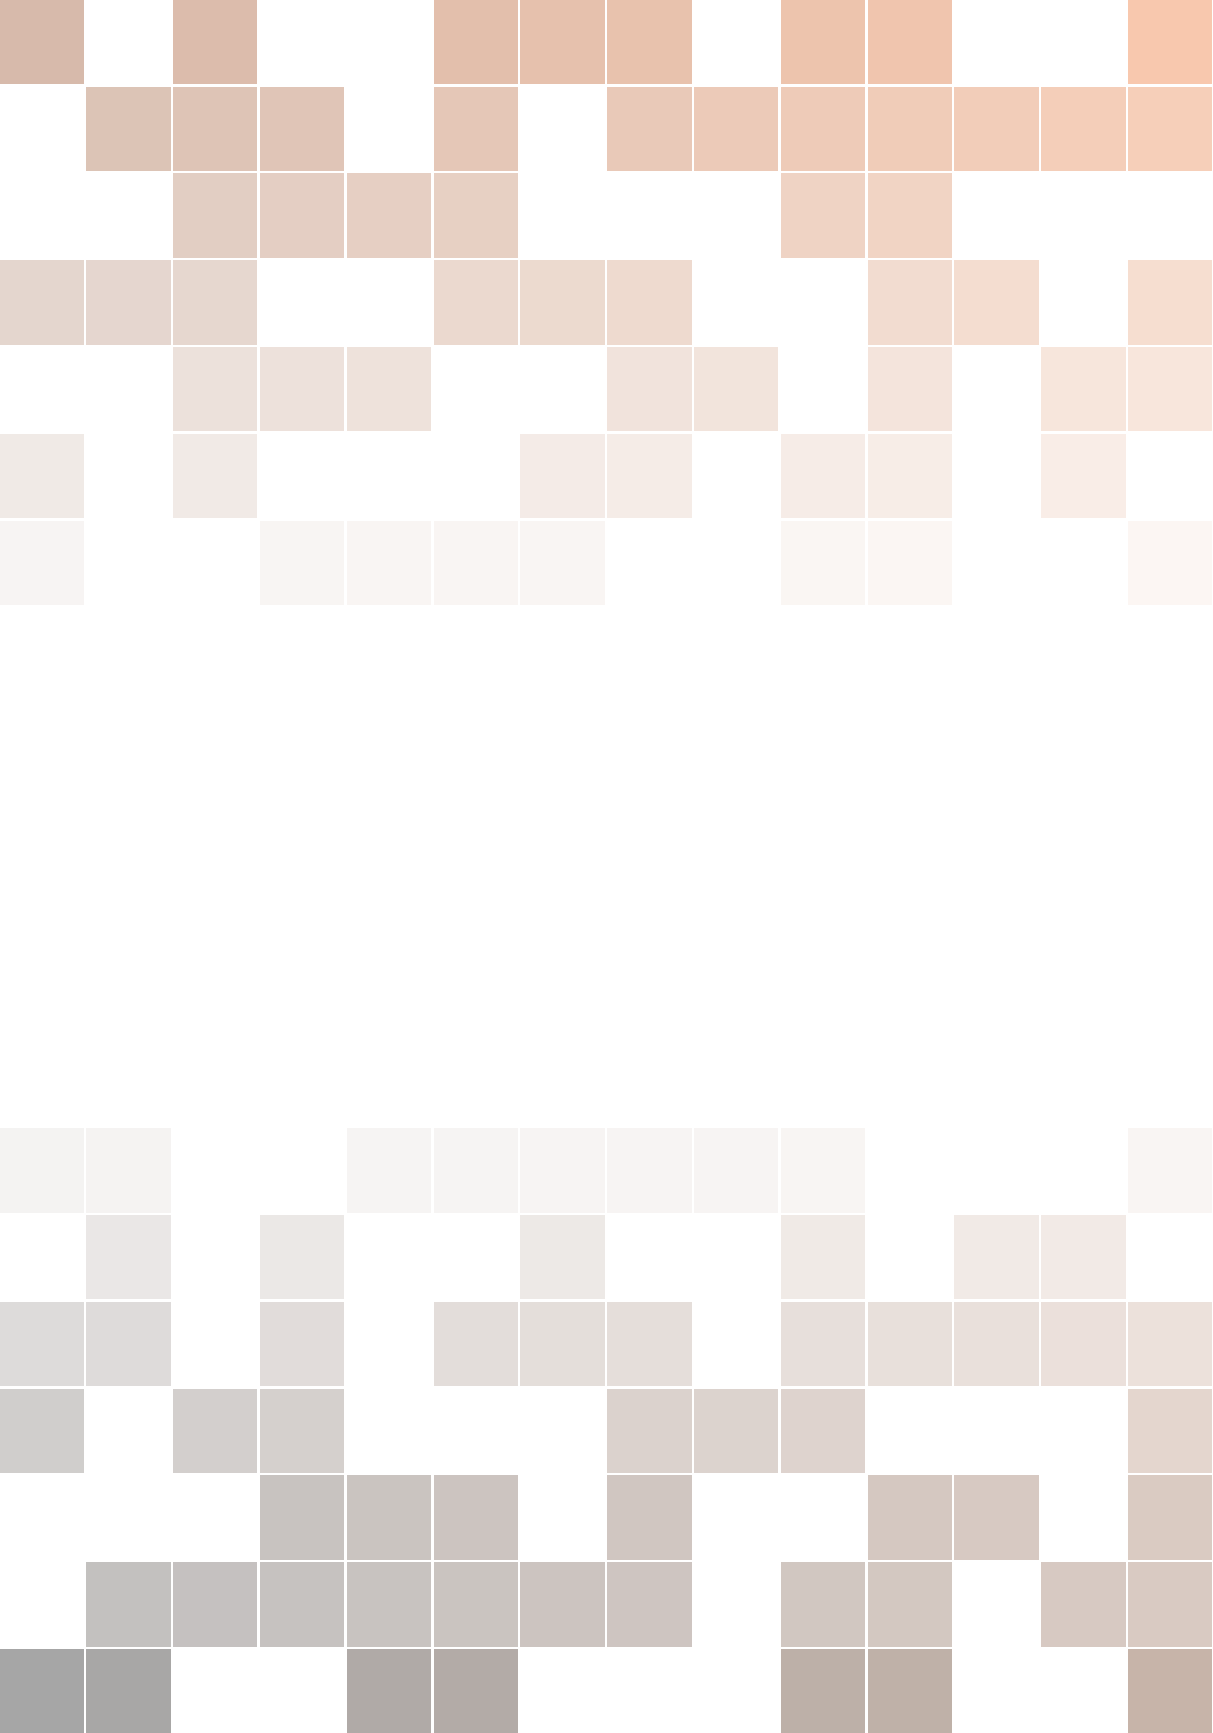
\includegraphics[scale=1]{background}}} % Image background
\par\normalfont\fontsize{15}{15}\sffamily\selectfont
“OpenQuake: Calculate, share, explore”
\centering
\vspace*{9cm}
\par\normalfont\fontsize{35}{35}\sffamily\selectfont
Testing procedures adopted in the development of the hazard 
component of the OpenQuake-engine\par % Book title
\endgroup

%----------------------------------------------------------------------------------------
%	COPYRIGHT PAGE
%----------------------------------------------------------------------------------------

\newpage
~\vfill
\thispagestyle{empty}

\noindent Copyright \copyright\ 2014 GEM Foundation\\ % Copyright notice

\noindent \textsc{Published by GEM Foundation}\\ % Publisher

\noindent \textsc{globalquakemodel.org/openquake}\\ % URL

\noindent 
   {\bf{Disclaimer}} \hfill \\
   This report is distributed in 
   the hope that it will be useful, but without any warranty: without 
   even the implied warranty of merchantability or fitness for a 
   particular purpose. While every 
   precaution has been taken in the preparation of this document, in 
   no event shall the authors of the manual and the GEM Foundation be 
   liable to any party for direct, indirect, special, incidental, or 
   consequential damages, including lost profits, arising out of the 
   use of information contained in this document or from the use of 
   programs and source code that may accompany it, even if the authors 
   and GEM Foundation have been advised of the possibility of such damage. 
   The report provided hereunder is on as "as is" basis, and the authors 
   and GEM Foundation have no obligations to provide maintenance, support,
   updates, enhancements, or modifications. 
   \hfill \\
   %
   \vspace{0.4cm} \hfill \\
   {\bf{License}} \hfill \\
   This Report is distributed under the Creative Common License 
   Attribution-NonCommercial-NoDerivs 3.0 Unported (CC BY-NC-ND 3.0) 
   (see link below). You can download this Book and share it with 
   others as long as you provide proper credit, but you cannot change 
   it in any way or use it commercially. 
   \hfill \\

\noindent \textit{First printing, May 2014} % Printing/edition date

%----------------------------------------------------------------------------------------
%	TABLE OF CONTENTS
%----------------------------------------------------------------------------------------

\chapterimage{chapter_head_1.pdf} % Table of contents heading image

\pagestyle{empty} % No headers

\tableofcontents % Print the table of contents itself

\cleardoublepage % Forces the first chapter to start on an odd page so it's on the right

\pagestyle{fancy} % Print headers again

%----------------------------------------------------------------------------------------
%	CHAPTER 1
%----------------------------------------------------------------------------------------
\chapterimage{chapter_head_1.pdf} % Chapter heading image
\chapter{Introduction}
The current document describes the testing procedures adopted in 
the development of the hazard component of the \gls{acr:oqe}, the 
open source hazard and risk software developed by the Global 
Earthquake Model initiative.

Nowadays seismic hazard analysis serves different needs coming 
from a variety of users and applications. 
%
These may encompass engineering design, assessment of earthquake risk 
to portfolios of assets within the insurance and reinsurance sectors, 
engineering seismological research, and effective mitigation via public 
policy in the form of urban zoning and building design code formulation.

Decisions based on seismic hazard results may have impacts on
population, properties and capitals, possibly with important repercussions 
on our day-to-day life. For these reasons, it is recommendable that 
the generation of hazard models and their calculation is based on 
well-recognized, state-of-the-art and tested techniques, requirements 
that must be reconciled with the need to regularly incorporate 
recent advances given the progress carried out within the 
scientific community. 
%
The features described below contribute to fulfill these requirements: 
%
\begin{itemize}
    \item Software should have a modular and flexible structure capable to 
    incorporate new features and - as a consequence - offer to the users 
    the most recent and advanced techniques. 
    %
    In very general terms, modularity is the level to which a component 
    of a system can be moved, replaced or reused. 
    %
    In software design, modularity means the separation of the software
    into smaller independent components that can be implemented, maintained 
    and tested easily and efficiently.
    %
    \item Software should have and extensive test coverage which captures 
    possible errors and avoids regressions (i.e. unexpected behaviors 
    introduced by new features).
    %
    Software testing \parencite{myers2012} is an important, complex and 
    vast discipline which helps developing methods and processes aimed at 
    certifying the extent to which a computer code behaves according 
    to the original design and user specifications.
\end{itemize}
% . . . . . . . . . . . . . . . . . . . . . . . . . . . . . . . . . . . > Figure
\begin{figure}[!ht]
\centering
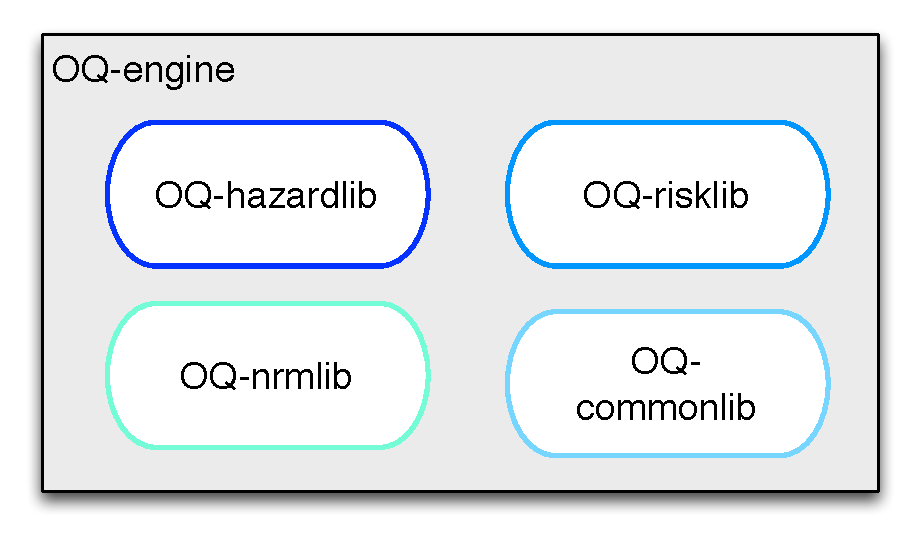
\includegraphics[width=9cm]{./Pictures/qa/oq-engine_structure.pdf}
\caption{A schematic describing the main components of the OpenQuake-engine 
    software.}
\label{fig:oqe_structure}
\end{figure}
% . . . . . . . . . . . . . . . . . . . . . . . . . . . . . . . . . . . < Figure
% 
The \gls{acr:oqe} includes different levels of modularity. 
The first is the one separating the engine itself into a number of 
libraries (see Figure \ref{fig:oqe_structure}) each one containing well 
identified knowledge, objects and methods (e.g. the OQ-hazardlib  
includes objects and methods needed to compute probabilistic 
seismic hazard). 
% 
The second one pertains to the data model adopted in the development 
of each library as a result of the abstraction process.
%
According to \textcite{berkes2012} scientific software must be:
\begin{itemize}
\item Error proof
\item Flexible and able to accommodate different methods
\item Reproducible and re-usable. 
\end{itemize}
%
% ..............................................................................
\section{Testing and Quality Assurance}
Despite the distinction between software testing (in some cases also called 
Quality Control) and \gls{acr:sqa} is vague and partly open to personal 
judgment, it's clear that \gls{acr:sqa} is a more comprehensive and 
overarching process than software testing. 
%
\gls{acr:sqa} aims at the definition of the best processes  
that should be used to provide guarantees that user expectations will 
be met. 
% 
Software testing focuses instead on detecting software faults by inspecting 
and testing the product at different stages of development.
%
% . . . . . . . . . . . . . . . . . . . . . . . . . . . . . . . . . . . . . . . 
\subsection{Testing}
Software testing can be implemented at different stages of the development 
process, with varying strategies to approach the problem.
%
The \gls{acr:oqe} and the associated libraries are developed following an 
agile paradigm. This development strategy is organized in a way that 
the creation of the real code is completed in parallel and fully 
integrated with the software testing process.

The software engineering community provides a wide range of testing levels
and typologies. In the current document we consider just a portion of them
with the specific intent to illustrate the standards used in the 
development of the \gls{acr:oqe} and particularly of its hazard component.
%
% . . . . . . . . . . . . . . . . . . . . . . . . . . . . . . . . . . . . . . . 
\subsection{Quality Assurance}
From the IEEE ``Standard for Software Quality Assurance Processes'':
\emph{Software quality assurance is a set of activities that define and 
assess the adequacy of software processes to provide evidence that establishes 
confidence that the software processes are appropriate for and produce 
software products of suitable quality for their intended purposes. 
A key attribute of SQA is the objectivity of the SQA function with 
respect to the project. The SQA function may also be organizationally 
independent of the project; that is, free from technical, managerial, 
and financial pressures from the project.} In this document we are not 
covering topics related to \gls{acr:sqa} since this would go beyond its
scopes.  
%
% ..............................................................................
\section{Document structure}
The document is organized into four main chapters and two appendixes.
 
In the current chapter we provide a very brief and general introduction 
to software testing with a focus on the testing of scientific software. 
 
In the second chapter we describe the module, or unit, testing, 
the acceptance tests adopted in the development of the 
\gls{acr:oqe} and we discuss some examples. 
 
In the third and fourth chapters we illustrate tests comparing 
the results computed with the \gls{acr:oqe} against the ones 
computed using different probabilistic seismic hazard analysis 
software.
  
Appendix \ref{sec:app1} provides details on the PEER tests 
implemented in the \gls{acr:oqhl}.

%----------------------------------------------------------------------------------------
%	CHAPTER 2
%----------------------------------------------------------------------------------------
\chapterimage{chapter_head_1.pdf} % Chapter heading image
\chapter{Unittesting}
\section{Unit-Testing: An Overview}

At the first level of the code quality assurance process is the practice of ``unit-testing''. This process is a central tenet of test-driven software development and is widely established as a means of ``best-practice''. Before looking closely at the OpenQuake approach to unit-testing it is important to establish what are the precise objective of the unit-testing process and the benefits (and limitations) that it brings.

\subsubsection{Correctness of Implementation}

This objective is obviously the primary goal of unit-testing, to ensure that each function of the code is operating in the manner expected by the developer. ``Correctness'', in this case, requires that the function produces both the correct output, but also if there are cases in which function may fail then the means of failure should be predictable. The following is a relatively simple example of how a unit-test relates to a function:

Consider a simple function to multiply two numbers and take the logarithm of the result. A relevant analogy may be that of a magnitude scaling relation calculation, in which both a rupture length and rupture width are required, and the logarithm of the area may be needed by the function itself. In this circumstance a negative value in either of the two inputs would result in a calculation error. This could be coded in the following manner. 

\begin{lstlisting}[frame=single]
def get_log_area(length, width):
    if (length < 0) or (width < 0):
        raise valueError("Both inputs must be positive")
    else:
        return log10(length * width)
\end{lstlisting}

From the description above it is evident that the user requirements inform the manner in which the function should behave (i.e. negative values cannot be tolerated). To ensure that the function is operating correctly, we wish to write a set of tests that will confirm the behaviour is correct:

\begin{enumerate}
\item 1. If both $a$ and $b$ are equal to 10.0, then the function should return 2.0

\item If $a = -1$ and $b = 10$ the function should raise an error reporting the stated message ``Both inputs must be positive''.

\item If $a = 10$ and $b = -1$ the function should raise an error reporting the stated message ``Both inputs must be positive''.

\item If $a = -1$ and $b = -1$ the function should raise an error reporting the stated message ``Both inputs must be positive''.
\end{enumerate}

A unit-test for this function is an additional function that will check that both cases are satisfied, and will report an error if not. 

A comprehensive unit-test suite for a software may fulfil two objectives: \textbf{line coverage} and \textbf{parameter coverage}. The former should ensure that, in as far as possible, every line (or statement) in the code is executed as some point in the testing process. The latter should ensure that the behaviour of the function is predictable when supplied with ``unusual'' parameters. In the above example, both objectives are satisfied by the tests. The first test will result in a positive valued ``area'', thus executing the second branch of the logical path, the second test will result in a negative area and will execute the first logical branch. Therefore all lines of the code are covered and the line coverage is complete. We also see that in this simple example there are four possible cases: i) a is positive and b is positive, ii) a is positive and b is negative,  ii) a is negative and b is positive, and iv) both a and b are negative. Only the first case is valid, therefore the first test ensures that they provide the correct answer (usually verified by independent means), whilst the remaining tests should ensure that the function raises the correct error. Thus the full parameter space of the input is ensured.

The above case is, of course, trivial; however, as shall be seen in due course, this same process can be applied in more complex contexts. Furthermore, the same unit-testing approach can be applied not only to individual components within the PSHA calculation, but also to full calculations, essentially verifying that the hazard curve produced by the full PSHA calculator is in agreement with that produced independently (sometimes by hand).

\subsubsection{Identifies Problems Prior to Software Release}

This advantage is largely self-explanatory, but for many software projects this can reduce the possibility of requiring \emph{a posteriori} fixes to the code (patches). By compiling a comprehensive suite of unit-tests, and following a software development and release process that should automatically run the tests at the point of packaging, this should ensure that new features added to the software cannot inadvertently break other components.

\subsubsection{Facilities Improvements in Performance}

In the creation of software intended to perform demanding scientific calculations, like those commonly associated with PSHA, the issue of computational performance and efficiency is a major one. There is a continuing need to improve the speed and reduce the work required to undertake the PSHA calculation. To implement improvements it is necessary to ensure that optimisations do not modify the outputs of the calculation, only the speed at which they are performed. The unit-testing is absolutely fundamental to this process as optimisation cannot be undertaken readily without a means to ensure the calculation outputs have not changed. This point was a critical motivation behind the transition from the OpenSHA basis of the OpenQuake hazard calculation engine prior to version 1.0, to the current OpenQuake hazard library.

\section{Continuous Integration}

OpenQuake is developed and packaged within a ``continuous integration'' system (\href{https://ci.openquake.org/}{https://ci.openquake.org/}), which used the open-source software ``Jenkins'' (\href{http://jenkins-ci.org/}{http://jenkins-ci.org/}). Continuous integration is used in large software projects to run a full test suite of the complete software, either at fixed time intervals or, as in the current case, when any new code is committed to the repository. The continuous integration system will do the following:

\begin{enumerate}
\item Run the full set of unit-tests for all code in all of the linked repositories. This will include the main (or ``master'') branch of the software repository, i.e. the one that will be used for packaging of the software, as well as some development branches.

\item Run a test of the software installation. This test will install the software on a dedicated platform and check that the installation of the software is successful. This test also ensures that if changes occur in the dependency packages, and these changes affect or compromise the installation and operation of the software, these problems are recognised immediately.

\item The software will also run standard Python tests for quality of code, compilation of documentation etc.

\item Several long-running tests may also be run. These implement larger scale seismic hazard and risk calculations designed to test the overall performance of the engine. 
\end{enumerate}

If at any point the tests should fail, the OpenQuake development team will be notified automatically. This should ensure that software that is failing any of the tests will remain on the main branch of the repository for the minimum amount of time possible. Furthermore, if the continuous integration tests fail, the new code will not be integrated into the nightly package of the software. 

\section{The OpenQuake Hazard Library: Unit Tests}

The unit-test suite for the OpenQuake hazard library consists of three types of tests: i) simple tests for individual functions to verify the correctness of implementation (``component testing''), ii) simple tests of the full calculators for PSHA (``method testing''), and iii) ``acceptance'' tests, which provide a basic quality assurance check for the each of the three main calculators. 

\subsection{Component Testing}

The unit-testing at the component level breaks the functions into simple calculations whose results can be verified by hand. These tests, similar in nature to that illustrated previously, provide the majority of the line and parameter coverage needed to ensure a robust code. To illustrate the comprehensive nature of the coverage we consider the example of the functions to undertake calculations of geodetic distance between two points, which can be found here: \href{https://github.com/gem/oq-hazardlib/blob/master/openquake/hazardlib/geo/geodetic.py}{https://github.com/gem/oq-hazardlib/blob/master/openquake/hazardlib/geo/geodetic.py}. Whilst not necessarily a complex function in itself, the distance between two points on the Earth's surface is a critical component of the software that is frequently called at several points of the PSHA process. Therefore, it is critical that the function operates correctly and its behaviour under extreme cases is understood. Thus, this relatively simple function is verified in the following cases:

\begin{itemize}
\item \verb=test_LAX_to_JFK= Checks that a correct geodetic distance is calculated for two known locations on the Earth. This value is verified against an implementation of the algorithm provided by an online geodetic calculation tool.
\item \verb=test_on_equator= Checks that the correct distance is provided for two points located on the equator.
\item \verb=test_along_meridian= Checks that the correct distance is returned for two points located along the same meridian.
\item \verb=test_one_point_on_pole= Verifies the distance calculations for two points assuming one point is located at the geographic pole.
\item \verb=test_small_distance= Verifies that two points separated by a distance within the floating point error are considered to be separated by zero km
\item \verb=test_opposite_points= Verifies the correct distance between two points in different longitudinal hemispheres (i.e. checks that the distance crosses the international dateline correctly).
\item \verb=test_array= Verifies the correct distances between two set of points
\item \verb=test_one_to_many= Verifies the correct distances between one point and a set of points.
\end{itemize}

The test suite for this one function is illustrative of several key components of the unit-testing. First is the use of an independent tool to provide the expected values of the calculation under simple conditions. Second is the use of ``extreme cases'' such as polar locations, or across the International Dateline. These ensure that the function can be global in application. 

The nature of the interdependencies between the functions also means that one a functions own unit-test is verified, the function can then form the basis for testing other conditions. So for example, the geodetic distance tools also contain a method to calculate the minimum distance between a collection of points and a single point. Rather than requiring new expected distances for the different conditions, the geodetic distance function can then be used to construct tests for functions that utilise it. This makes the testing process more efficient, and reduced the need to write large numbers of tests in order to ensure correct behaviour of the function.

\subsection{Ground Motion Prediction Equation (GMPE) Testing}

The implementation process for ground motion prediction equations requires careful consideration, as it is in this area that new features may be expected to be added regularly, and where contributions from third parties are more likely to be incorporated into the software. Furthermore, in most cases the expected values of the functions may only be obtained from independent implementations of the GMPE. These expected values take the form of test tables, which are simple comma-separated value (csv) files that provide the expected values and standard deviations of the ground motion prediction equation for an exhaustive combination of parameters for the predictor variables. These should be sufficient to ensure that every part of the GMPE is covered within the test. An example test table is shown in Figure \ref{fig:gmpe_test_table}.

\begin{figure}[htbp]
  \centering
  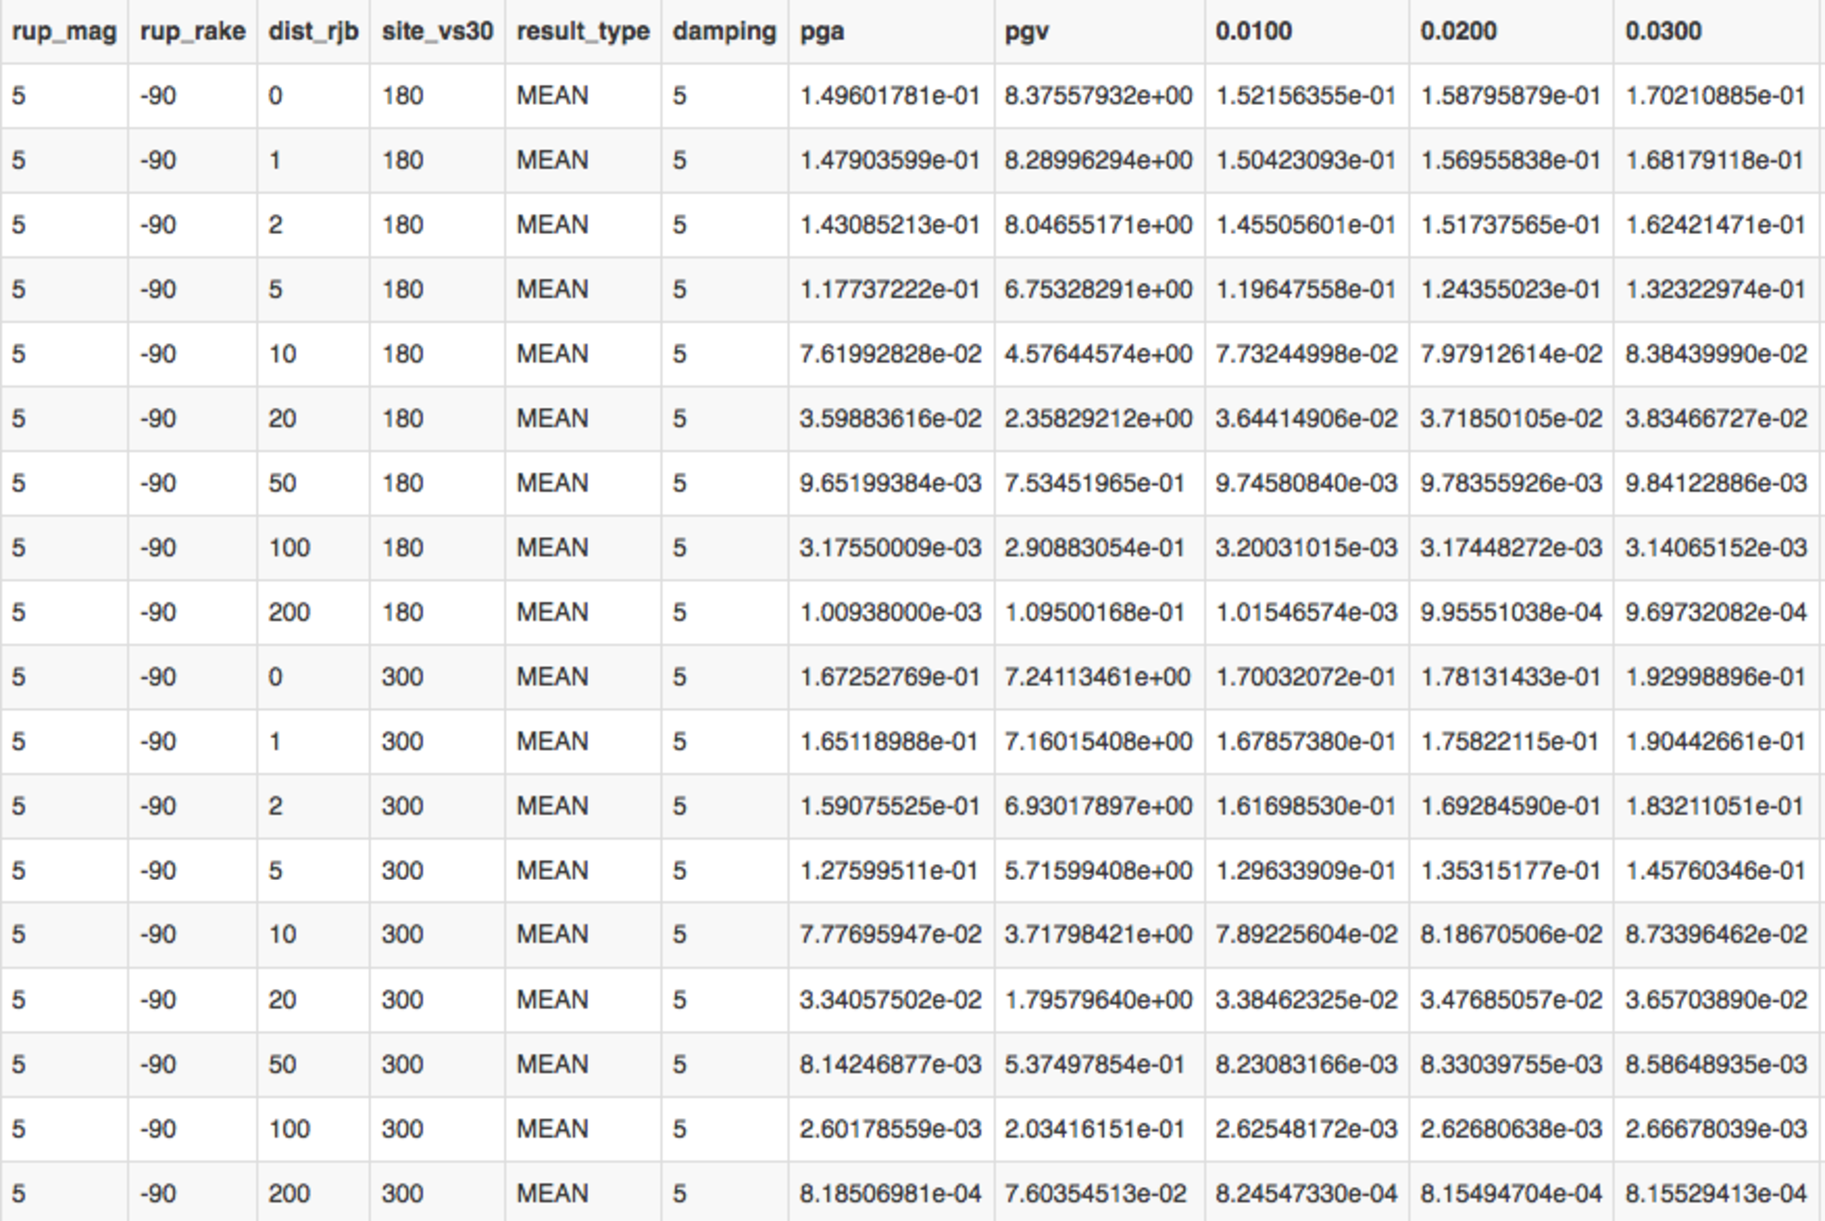
\includegraphics[width=0.8\textwidth]{./qareport/pictures/test_tables_screen_capture.pdf}
  \caption{Example GMPE test table used by OpenQuake}
  \label{fig:gmpe_test_table}
\end{figure}

To ensure the most objective testing strategy, we aim for the test tables to match the GMPE creator's own implementation of the GMPE, in as far as possible. Therefore we prefer to solicit input from the authors of the GMPE. This will often take one of two forms. We ask that the authors can provide test tables, in a convenient format, or that they provide their own software implementation of the GMPE, from which we will then generate the test tables. Input from the GMPE authors is highly desirable within this process as it can help resolve issues that are perhaps ambiguous within the original publications of the GMPE and it can identify errors and bugs in the author's own implementation. The full workflow for GMPE implementation in OpenQuake is shown in Figure \ref{fig:gmpe_flowchart}.

\begin{figure}[htbp]
  \centering
  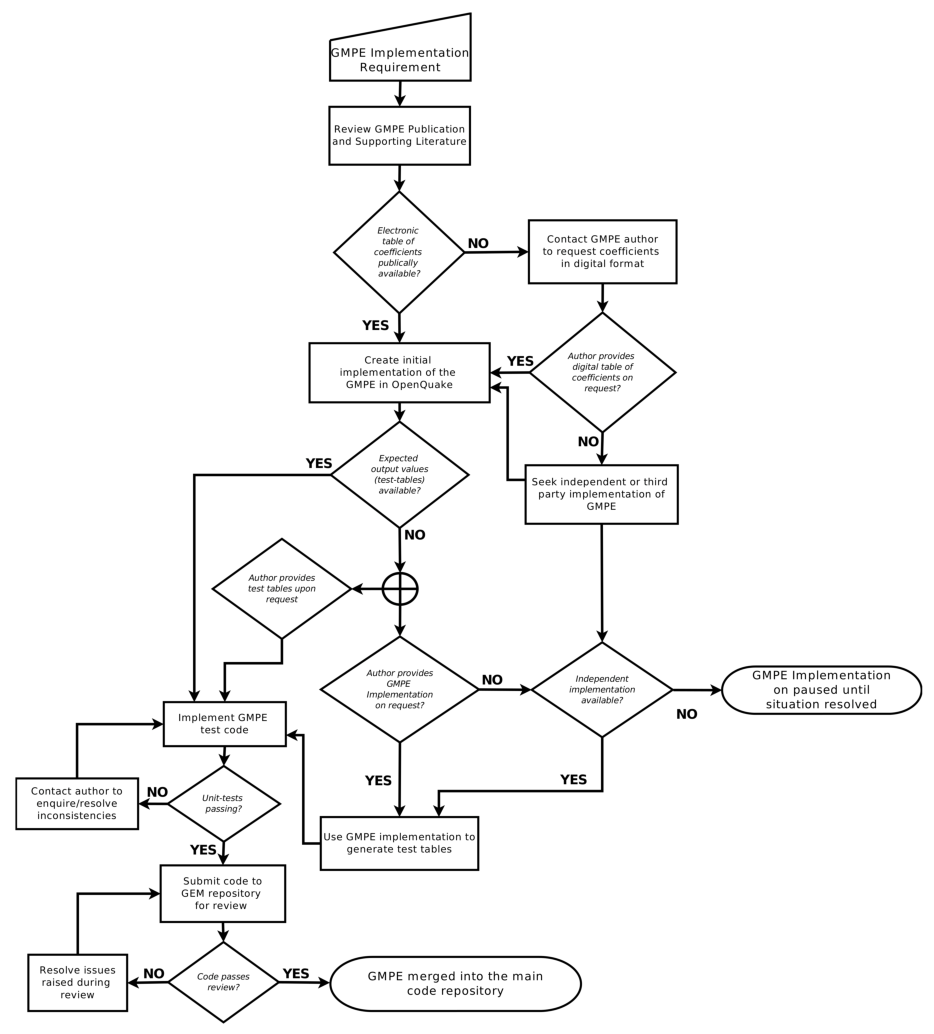
\includegraphics[width=\textwidth]{./qareport/pictures/gmpe_implementation_flowchart.pdf}
  \caption{OpenQuake GMPE Implementation Process}
  \label{fig:gmpe_flowchart}
\end{figure}

The GMPE unit-tests themselves are designed to be simple for the user to create once the test tables are provided. Ideally the expected values should match the implementation values to within the test precision (typically permitting a difference of $10^{-7}$). In some cases, however, it may not be possible to match the desired level of precision and therefore the tests permit the maximum discrepancy level (as a percentage) to be specified. Discrepancies may arise due to rounding of the coefficients within published tables, but ideally the tolerable discrepancy between an expected and predicted value should be not more than one tenth of one percent.

As is shown from Figure \ref{fig:gmpe_flowchart}, once the GMPE test tables are created, the GMPE implementation should then be checked against the unit-tests. If discrepancies cannot obviously be resolved the author may then be contacted for clarification. Once the unit-tests pass the code is then submitted for review by (typically) one or more of the software development team and one or more of the scientific team. This may help identify issues such as inefficiencies or unclear code. Once the submission is accepted by both the scientific and IT reviewer the code is merged into the main repository. This will then trigger a full test from the continuous integration system described previously.


\section{Acceptance Tests}

In addition to the individual unit-tests on functions, the OpenQuake hazard library contains three code ``acceptance'' tests. These are tests that are designed to exercise the full workflow of the classical, event-based and disaggregation calculators. Further comprehensive tests of all of the main OpenQuake calculators are also found in the test suite of the main OpenQuake engine, and these shall be elaborated upon in section ??.

\subsection{Classical PSHA Acceptance Tests}

The following tests, taken from the PEER tests suite \citep{thomas2010}, are used as the the basis for the unit tests of the classical PSHA calculation engine:

\begin{enumerate}
\item \textbf{Set 1 Case 10} 

This test considers one uniform area source with a truncated exponential model with $M_{min}$ of 5.0, $M_{max}$ 6.5, b-value of 0.9 and an annual rate $M_W \geq M_{min}$ of 0.0395. As OpenQuake defines finite rupture planes for each of the points considered in the area source, the scaling relation was fixed such that the area of the finite rupture was equal to 1.0 km. Hypocentral depth is fixed at 5 km. The preferred GMPE is \cite{sEtAl1997} for rock, with sigma set to 0.0. The expected values for the unit tests are those provided in the appendix of \cite{thomas2010} (page A - 15), which represent the mean values of the distribution of estimates from the software considered. As these are not solved by hand, the test are considered to pass when the following condition is satisfied for all values:

\begin{equation}
|calculated - expected| \leq \left( {atol + rtol * |expected|} \right)
\end{equation}

where $atol$ and $rtol$ are the absolute and relative difference between two terms, set to $10^{-4}$ and $10^{-1}$ respectively.

\item \textbf{Set 1 Case 11}

The same area source and GMPE are considered as for \textbf{Set 1 Case 10}; however, the hypocentral depth is distributed uniformly between 5 km and 10 km. All other conditions are the same.


\item \textbf{Set 1 Case 2}

This case considered a vertical strike-slip planar fault rupture with a single magnitude $M_W$ 6.0, whose expected rupture plane is smaller than the total area of the fault. The slip rate is assumed to be $2 mm yr^{1}$, giving an annual recurrance of 0.0160425 $yr^{-1}$. The following scaling relations are used, which in combination give an expected aspect ratio equal to 2.0.

\begin{eqnarray}
\log_{10} A &=& M_W - 4.0\\
\log_{10} W &=& 0.5 M_W - 2.15\\
\log_{10} L &=& 0.5 M_W - 1.85
\end{eqnarray}

where $A$, $W$ and $L$ are the rupture area, width and length respectively. The GMPE, site condition and sigma truncation are the same as for \textbf{Set 1 Case 10} and \textbf{Set 1 Case 11}


\item \textbf{Set 1 Case 5}

This case considers the same fault plane as in \textbf{Set 1 Case 2} albeit with an exponential magnitude frequency distribution with $M_{MIN}$ and $M_{MAX}$ of 5.0 and 6.5 respectively and a b-value of 0.9. The same slip rate is assumed, which translates into an a-value of 3.1292. All other inputs are the same.
\end{enumerate}


\subsection{Event-Based PSHA Acceptance Tests}

The event-based acceptance tests are designed to verify that for a sufficiently long stochastically generated catalogue originating from an area source, $10^6$ years in this case, the normalised rate of events in each magnitude frequency bin is approximately equal to that of the expected magnitude frequency distribution. This is expanded to check out source to site distance filtering by considering a second source beyond the expected soure-to-site distance filter range. 

\subsection{Deaggregation Acceptance Tests}

The disaggregation calculator is tested in two separate places. A first unit-test evaluates the disaggregation of hazard for a simple case in which the probabilities in the disaggregations bins have been calculated, by hand, for a simple rupture model. This unit-test will fulfil the requirements of line and parameter coverage, including edge cases such as if the rupture crosses the international dateline, or if no ruptures contribute to the hazard at the site. A second unit-test using a more realistic source and GMPE combination are then implemented. In this case it is not possible to calculate the probabilities by hand, but instead the OpenQuake results are used as the expected values. This test is circular in nature, and is intended simply as a means to ensure that changes to the code do not alter the results of the disaggregation calculator.

\section{Summary}

In this section we have outlined both the process and the key benefits of developing comprehensive unit-tests for OpenQuake, as well as outlining the operation of the continuous integration system, which should ensure that code with the potential to break the tests cannot be packaged and released. The unit-tests themselves have not been discussed in detail as nearly one thousand tests are executed during the unit-test process. However, to view the comprehensive set of tests reader is encouraged to refer to the full test-suite, which is open and available on the OpenQuake code repository (\href{https://github.com/gem/oq-hazardlib/tree/master/openquake/hazardlib/tests}{https://github.com/gem/oq-hazardlib/tree/master/openquake/hazardlib/tests}). Furthermore, we have also discussed how OpenQuake development tries to facilitate correct implementation of features such as ground motion prediction equations. For relatively simple conditions, a selection of PEER tests \citep{thomas2010} are built into the testing process, making OpenQuake unique amongst other hazard software in integrating the verification into the development process. The following chapters will expand in greater detail upon the additional hazard curve benchmark tests, which both follow and expand upon the PEER testing process. T




%----------------------------------------------------------------------------------------
%	CHAPTER 3
%----------------------------------------------------------------------------------------
\chapterimage{chapter_head_1.pdf} % Chapter heading image
\chapter{Other PSHA codes: simple cases}
This chapter presents a number of benchmarks used to compare the OpenQuake-engine
hazard results against solutions provided by alternative software. The focus is on simple test cases which involve a single source typology at a time and no epistemic uncertainties. The end goal is to investigate discrepancies in modeling the same source typolgy in different software. Classical PSHA results (i.e. hazard curves and maps) generated by the OpenQuake-engine are compared against solutions computed using the the suite of seismic hazard analysis computer programs developed by the United States Geological Survey - National Seismic Hazard Program (USGS-NSHMP).
% ..............................................................................
\section{Comparison against the USGS-NSHMP computer programs}
The USGS-NSHMP developed a number of Fortran-based computer programs used to implement the U.S. national seismic hazard model (\cite{petersen2008}). Source codes are available on the internet (http://earthquake.usgs.gov/hazards/products/conterminous/2008/software/) together with input files containing the seismic hazard model definition. Input files are available for the three main source typologies
defined in the U.S. national seismic hazard model: distributed seismicity, crustal faults and subduction faults.
The USGS-NSHMP seismic hazard software offers therefore an excellent opportunity to test the OpenQuake-engine algorithms for the different seismic source typologies.

\subsection{Benchmarks for distributed seismicity}
As a benchmark for the modeling of distributed seismicity we selected a gridded seismicity model developed for the State of California (Figure \ref{fig:cal_grid}). The model is associated with the USGS-NSHMP computer program for gridded seismicity \textit{hazgridXnga3.f}. 

\begin{figure}[htb]
\centering
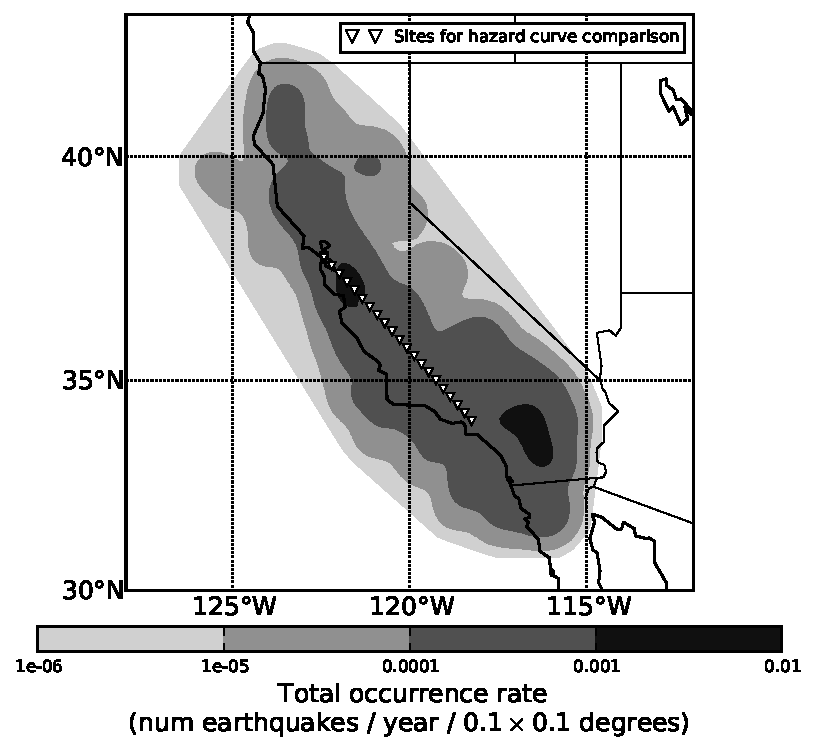
\includegraphics[width=12cm]{./qareport/pictures/CAmapC_21.pdf}
\caption{Gridded seismicity model used as benchmark for testing distributed seismicity in the OQ-engine. Hazard curves are compared for a set of 21 sites defining a profile connecting San Francisco to Los Angeles.}
\label{fig:cal_grid}
\end{figure}

\begin{figure}[!ht]
\centering
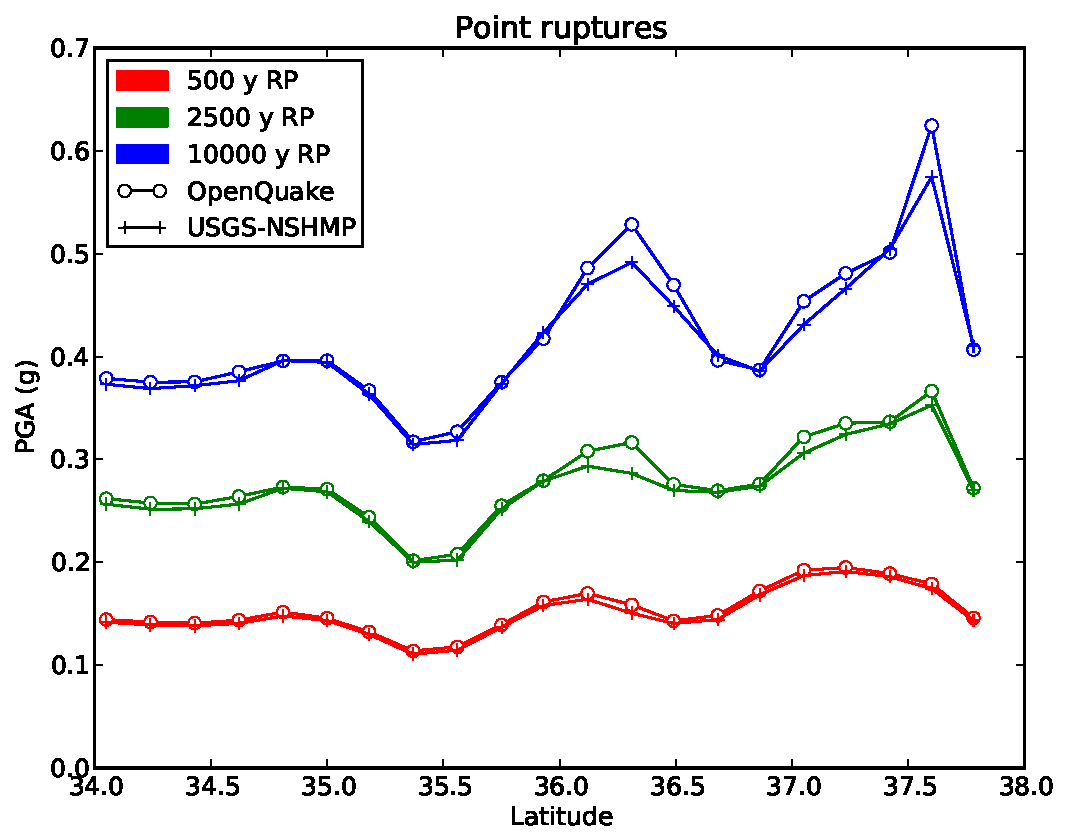
\includegraphics[width=12.5cm]{./qareport/pictures/gridded_seismicity_oq_nshmp_point.pdf}
\caption{Comparison of hazard map values for different return periods (RP) along the profile assuming \textit{point ruptures}}
\label{fig:cal_grid_map_point}
\end{figure}

\begin{figure}[!h]
\centering
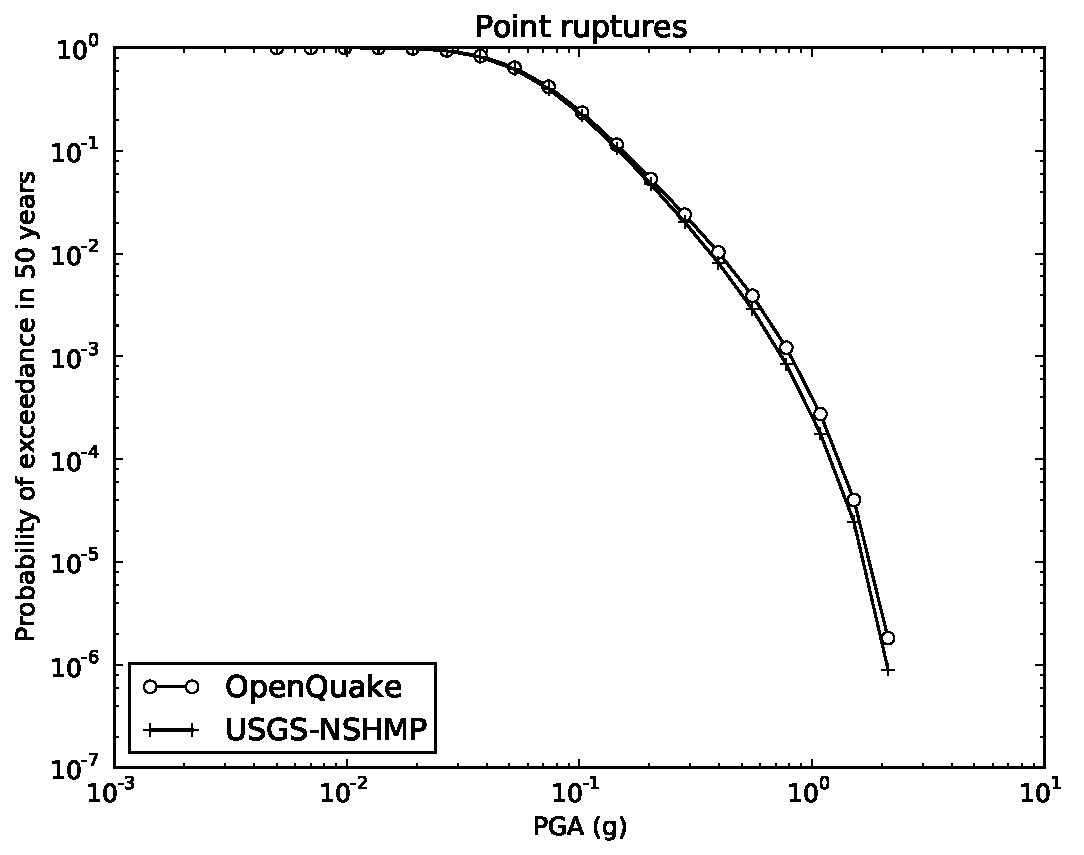
\includegraphics[width=12.5cm]{./qareport/pictures/-120pt7_36pt31_point.pdf}
\caption{Hazard curve comparison for site with coordinates -120.7E, 36.31N assuming \textit{point ruptures}}
\label{fig:cal_grid_curve_point}
\end{figure}

\begin{figure}[!ht]
\centering
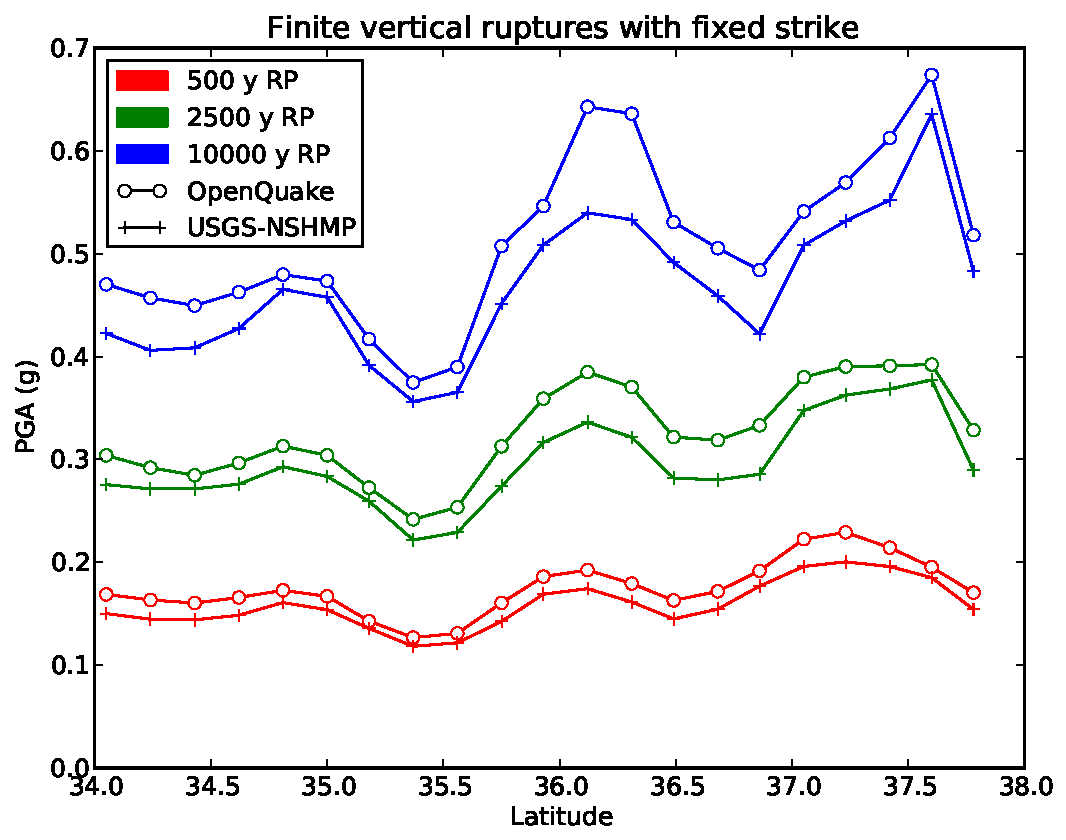
\includegraphics[width=12.5cm]{./qareport/pictures/gridded_seismicity_oq_nshmp_fixedstrikevertical.pdf}
\caption{Comparison of hazard map values for different return periods (RP) along the profile assuming finite vertical ruptures with fixed strike.}
\label{fig:cal_grid_map_finite}
\end{figure}

\begin{figure}[!h]
\centering
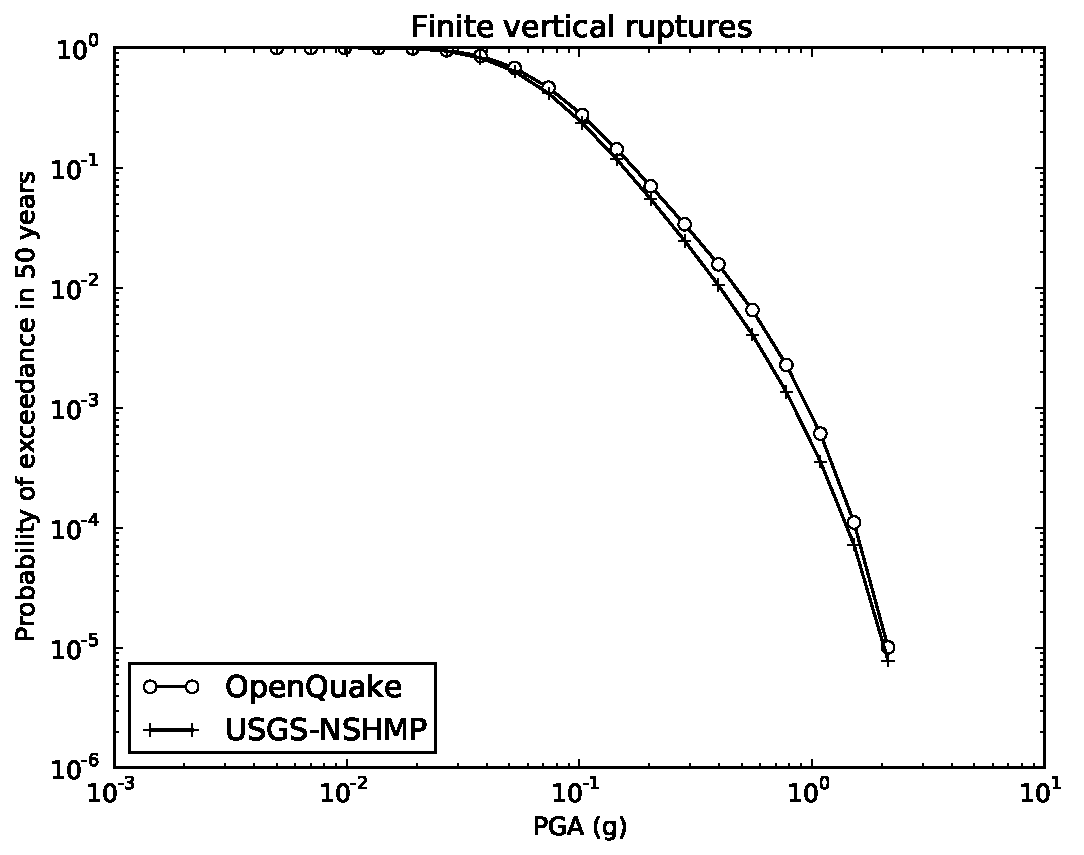
\includegraphics[width=12.5cm]{./qareport/pictures/-120pt7_36pt31_fixedstrikevertical.pdf}
\caption{Hazard curve comparison for site with coordinates -120.7E 36.31N assuming finite vertical ruptures with fixed strike.}
\label{fig:cal_grid_curve_finite}
\end{figure}

The model defines spatially variable occurrence rates over a regular grid (0.1 by 0.1 degrees) obtained using a smoothed seismicity approach (\cite{frankel1995}). Occurrence rates are defined from minimum magnitude equal to 5. Maximum magnitude is equal to 7 in areas away from faults. Close to faults, the maximum magnitude is assumed equal to the minimum between 7 and the fault's maximum magnitude. Occurrence rates follow a double truncated Gutenberg-Richter magnitude frequency distribution with $b_{GR} = 0.8$. Rupture extension is modeled using the magnitude-length scaling relationship of \citet{wells1994} for the 'All Slip Types' case ($L=10^{-3.22+0.69 M}$). The rupture top edge is placed at 0 km depth for $M \ge 6.5$ and at 5 km depth for  $M < 6.5$.

We compared hazard curves on a set of 21 equally spaced locations defining a profile connecting San Francisco (-122.42W, 37.78N) to Los Angeles (-118.25E, 34.05N). We computed hazard curves (probabilities of exceedance in 50 years) for peak ground acceleration using the \citet{boore2008} GMPE. This GMPE requires as distance metrics the Joyner-Boore distance ($R_{JB}$). 

We first computed hazard curves under the assumption of \textit{point ruptures}. That is ruptures are treated as having no spatial extension. Under this assumption $R_{JB}$ converges to epicentral distance. Results of the comparison (as PGA values for different return periods along the profile) are given in Figure \ref{fig:cal_grid_map_point}. Comparison of hazard curves at a single site is also given in Figure \ref{fig:cal_grid_curve_point}. For most of the locations, results are in agreement. For few sites, larger discrepancies are observed that increase with increasing return periods.

A second test is performed but considering extended ruptures. For simplicity, ruptures are assumed vertical and aligned along a single strike direction ($0^{\circ}$). All ruptures are assumed to be strike-slip. In the OQ-engine calculation, the rupture extension is modeled by considering the \textit{magnitude-area} scaling relationship of \citet{wells1994} ($A = 10^{-3.42 + 0.90 M}$) and assuming an aspect ratio equal to 1. In the \textit{hazagridXnga3.f} rupture extension is modeled based on the \textit{magnitude-length} scaling relationship of \citet{wells1994} ($L = 10^{-3.22+0.69 M}$).

Results of the comparison are given in Figures \ref{fig:cal_grid_map_finite} and \ref{fig:cal_grid_curve_finite}. Discrepancies are much larger than under the \textit{point ruptures} approximations, at all return periods. This can be motivated by the fact that the two software adopt different modeling strategies. The OQ-engine uses a magnitude-area scaling relationship which implies that rupture length may be increased if, for given area and rupture aspect ratio, the resulting rupture width is larger than the seismogenic layer thickness. On the contrary, in the USGS-NSHMP approach, rupture extension is constrained by a magnitude-length scaling relationship. For the same rupture magnitude, the OQ-engine may predict shorter distances and thus provide higher hazard values. For a more detailed analysis on the differences between the OpenQuake-engine and the USGS-NSHMP approach in modeling distributed seismicity we refer to the work of \citet{monelli2014}.

\subsection{Benchmarks for crustal faults}
As benchmarks for crustal faults, we considered two fault models for the State of California. One based on type-A faults (\cite{petersen2008}), which defines only characteristic fault sources (Figure \ref{fig:type_a_fault}) and one based on type-B faults (Figure \ref{fig:type_b_fault}), which contain mostly Gutenberg-Richter fault sources. Both source models are associated with the USGS-NSHMP computer program \textit{hazFXnga7c.f}.

Characteristic faults are defined through a Normal (i.e. Gaussian) magnitude-frequency distribution. For each magnitude-bin, the entire fault surface is assumed to rupture. In a characteristic model no scaling relationship is required, and hence floating ruptures are not modeled. On the contrary, in a Gutenberg-Richter fault, ruptures are floated only along the fault strike and rupture extension is modeled in terms of a magnitude-length scaling relationship. The magnitude-length scaling is actually derived from the magnitude-area scaling relationship of \citet{hanks2002} and assuming a fixed width (equal to the fault width).

% Type-A fault
\begin{figure}[!hb]
\centering
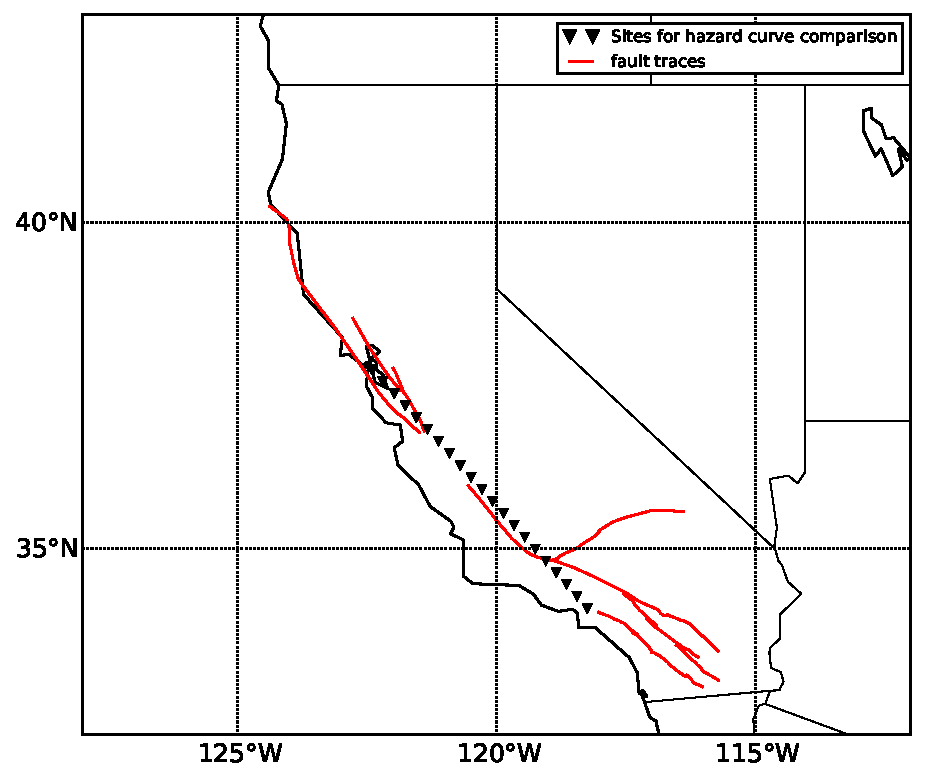
\includegraphics[width=12cm]{./qareport/pictures/aFault_aPriori_D2pt1.pdf}
\caption{Type-A fault model}
\label{fig:type_a_fault}
\end{figure}

% Type-B fault
\begin{figure}[!hb]
\centering
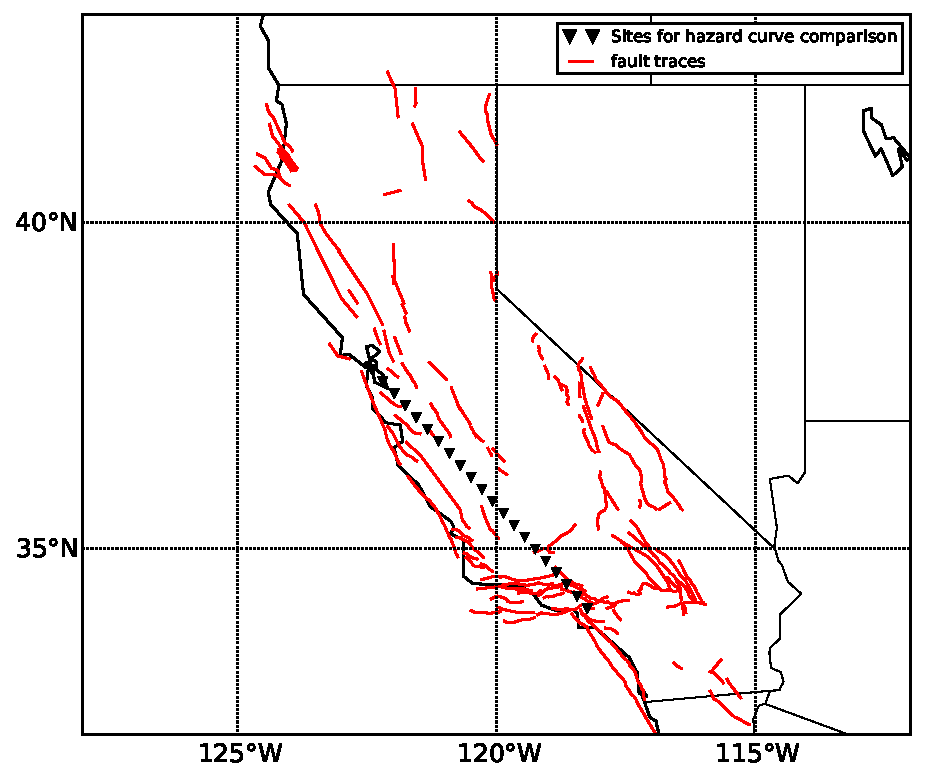
\includegraphics[width=12cm]{./qareport/pictures/bFault_stitched_D2pt1_GR0.pdf}
\caption{Type-B fault model}
\label{fig:type_b_fault}
\end{figure}

\begin{figure}[!ht]
\centering
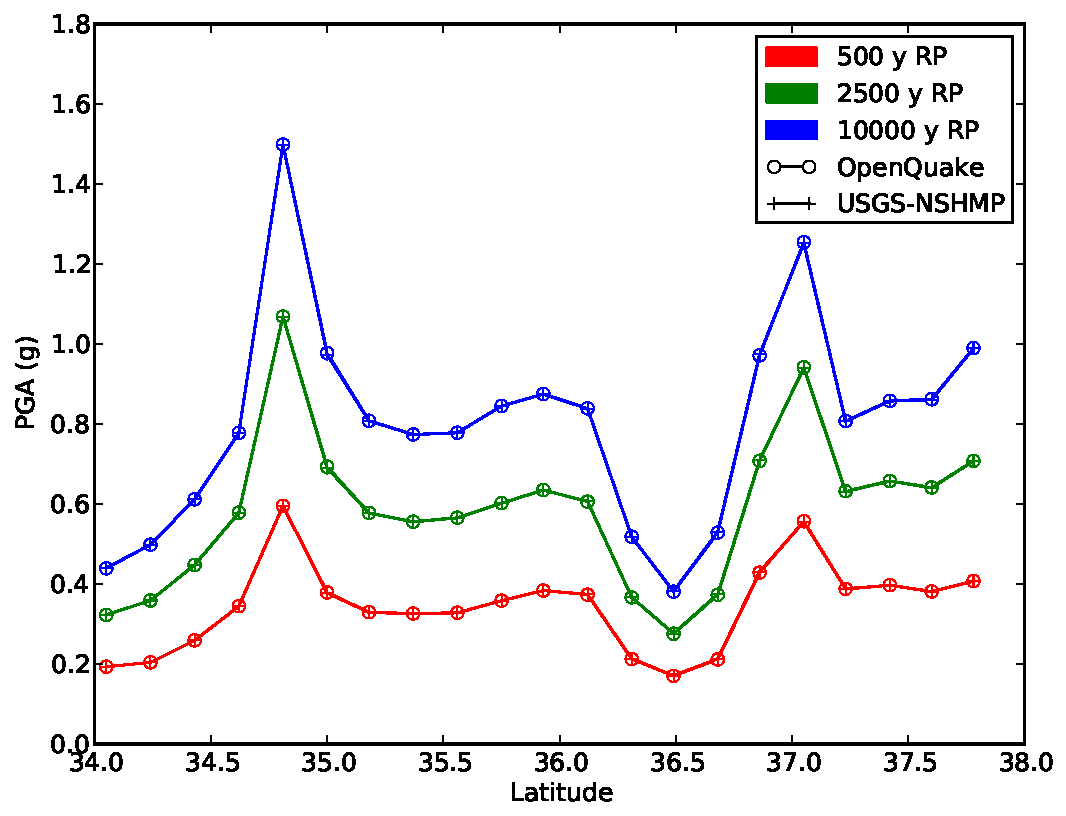
\includegraphics[width=12.5cm]{./qareport/pictures/oq_nshmp_aFault.pdf}
\caption{Hazard map comparison for Type-A fault model.}
\label{fig:type_a_map}
\end{figure}
\begin{figure}[!h]
\centering
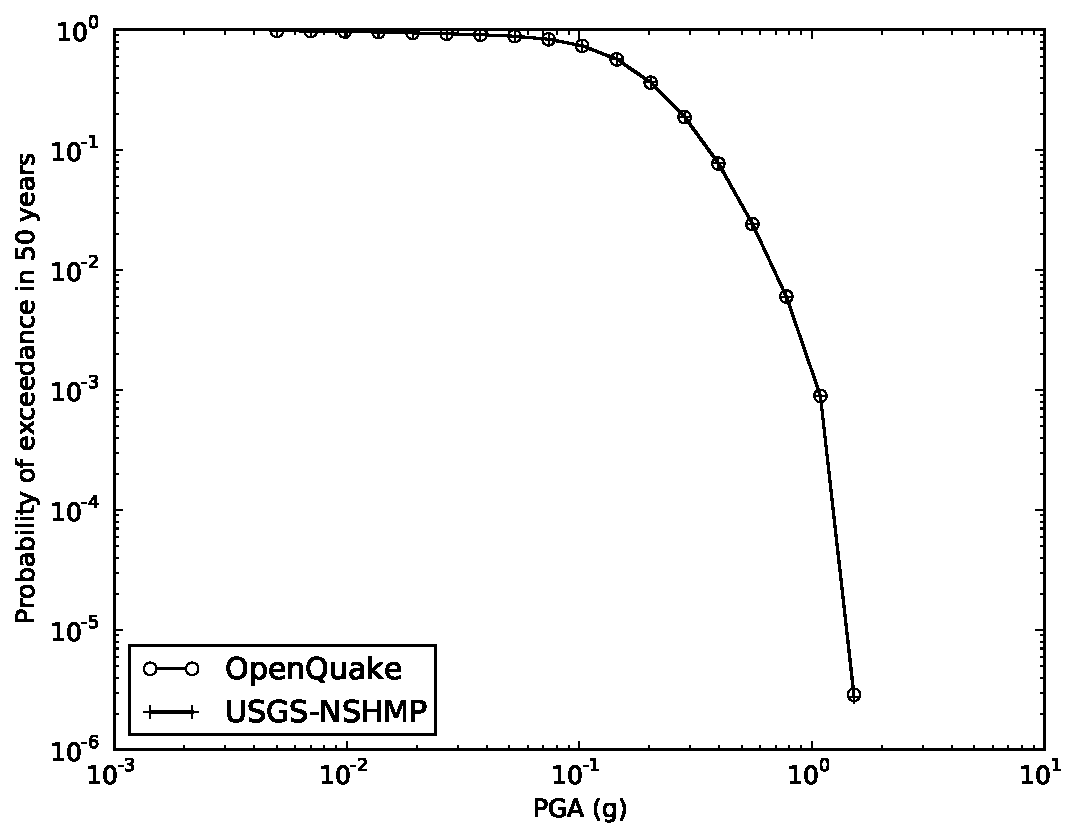
\includegraphics[width=12.5cm]{./qareport/pictures/-120pt49_36pt12_aFault.pdf}
\caption{Hazard curve comparison for site with coordinates -120.49E 36.12N using Type-A fault model}
\label{fig:type_a_curve}
\end{figure}

\begin{figure}[!ht]
\centering
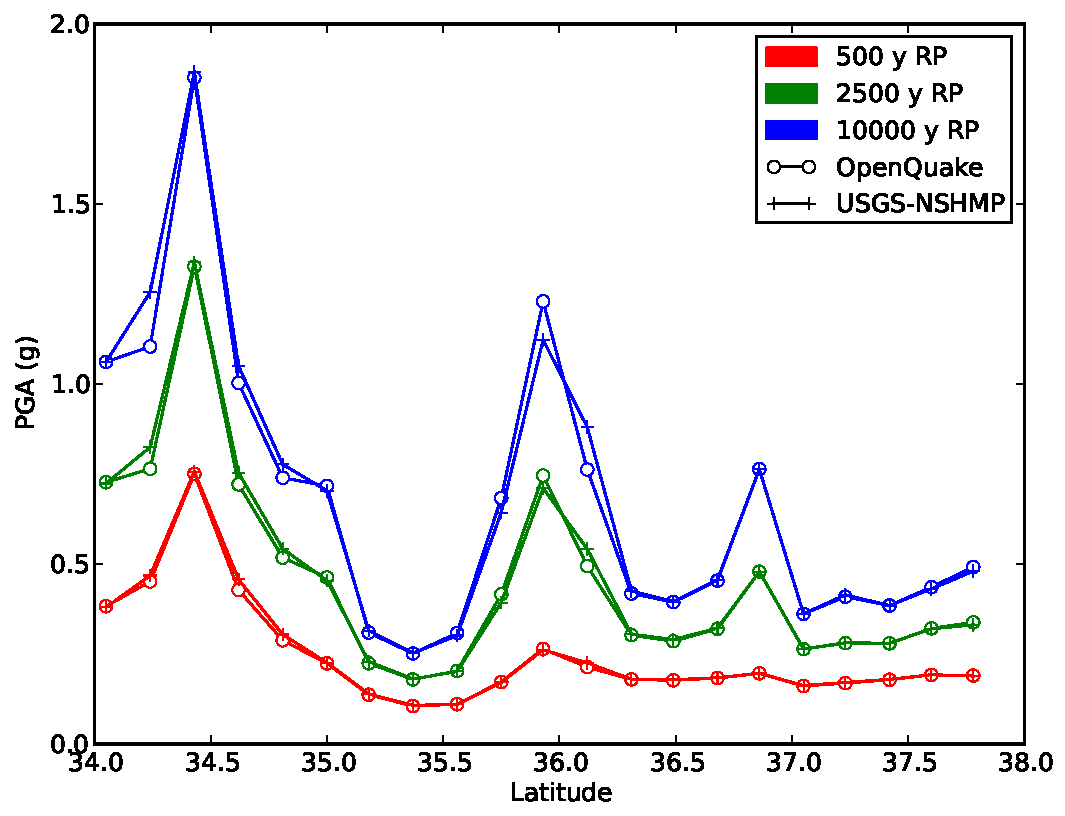
\includegraphics[width=12.5cm]{./qareport/pictures/oq_nshmp_bFault_ar1.pdf}
\caption{Hazard map comparison for Type-B fault model}
\label{fig:type_b_map}
\end{figure}
\begin{figure}[!h]
\centering
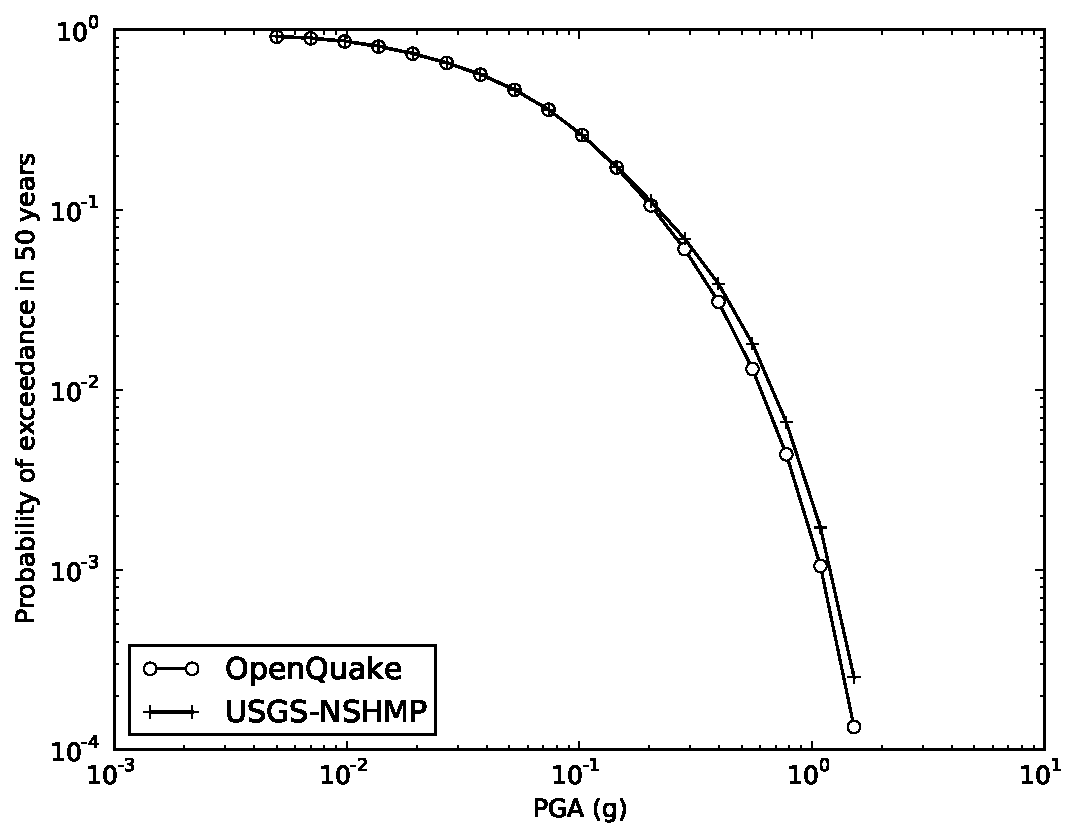
\includegraphics[width=12.5cm]{./qareport/pictures/-120pt49_36pt12_bFault_ar1.pdf}
\caption{Hazard curve comparison for site with coordinates -120.49E 36.12N using Type-B fault model}
\label{fig:type_b_curve}
\end{figure}

We compare hazard curves for the same set of locations as for the distributed seismicity model. Results of the comparison are given in Figures \ref{fig:type_a_map} and \ref{fig:type_a_curve} for the type-A fault model, and \ref{fig:type_b_map}, and \ref{fig:type_b_curve} for the type-B fault model. For the type-A fault model, the agreement between the USGS-NSHMP and OpenQuake-engine solutions is very good. When considering instead the results from the type-B fault model some discrepancies are visibile, especially for return periods longer than 500 years, altough the level of agreement is still acceptable. The lack of a complete agreement in the type-B fault model solutions may indicate the effect of differences in the rupture floating algorithm between the two software. In the OpenQuake-engine the magnitude-area scaling relationship of \citet{wells1994} is used and rupture floating occurs both along strike and dip. Indeed, the very good agreement in the case of the type-A fault model (which does not consider any rupture floating) confirms that the modeling of rupture extension and location on a fault surface plays an important role in the hazard calculation procedure.

\subsection{Benchmarks for subduction faults}
The 2008 U.S. national seismic hazard model (\cite{petersen2008}) defines fault sources with complex geometries to model large subdaction interface faults in the Cascadia region. We thus selected a fault model for the Cascadia region as a benchmark for the modeling of complex fault sources.

Similarly to what done for crustal sources, we considered a characteristic model (where earthquakes always rupture the entire fault surface) and an unsegmented model where ruptures (whose extension is constrained by a scaling relationship) are allowed to move along the entire fault surface. The characteristic model defines a single event of magnitude $M_{w}=9.2$ which breaks a complex fault surface depicted in Figure \ref{fig:cascadia_geo}. The unsegmented model defines the same fault geometry, however earthquake ruptures are generated from minimum magnitude 8.3 to maximum magnitude 8.7. Ruptures are floated only along the strike direction and rupture length is obtained from a magnitude-length scaling relationship specific for the Cascadia region. Both source models are associated with the USGS-NSHMP computer program \textit{hazSUBXnga.f}. To perfom a more fair comparison againt the OpenQuake-engine we modified the \textit{hazSUBXnga.f} code so that rupture length is computed from the \citet{wells1994} magnitude-area scaling relationship and assuming a rupture aspect ratio equal to 1.

Hazard curves are compared along two profiles, aligned along the E-W and N-S directions. When considering the characteristic model, the agreement between the solutions provided by the two software is very good (Figures \ref{fig:cascadia_char_ew}, \ref{fig:cascadia_char_ns}). On the contrary, when considering the unsegmented model (Figures \ref{fig:cascadia_float_ew} and \ref{fig:cascadia_float_ns}) large discrepancies are evident especially along the N-S profile. The large discrepancies can be understood again in terms of the differences between the rupture floating algorithm in the two software. In particular, the USGS-NSHMP code define rupture extension along length only and assume each rupture to extend along dip until the fault bottom edge. In the OQ-engine instead, rupture extension and shape is determined by a magnitude-area scaling relationship and rupture aspect-ratio, and each rupture can be moved both along strike and along dip. The bulge in the hazard map profiles as visible in Figure \ref{fig:cascadia_float_ns} can be explained in terms of a large number of ruptures modelled by the OQ-engine in the inner part of the fault surface. In the USGS-NSHMP approach, the number of ruptures along the fault surface is constant, as also demonstrated by the constant hazard values along the N-S profile.
\begin{figure}
\centering
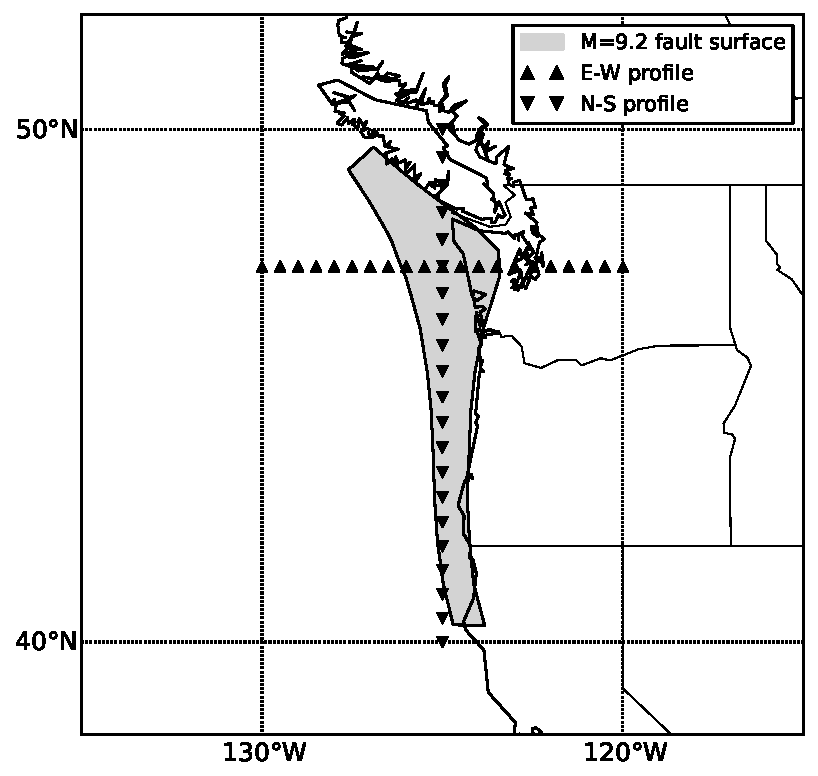
\includegraphics[width=12cm]{./qareport/pictures/cascadia_char.pdf}
\caption{Cascadia characteristic fault model ($M_{w}$=9.2)}
\label{fig:cascadia_geo}
\end{figure}

\begin{figure}
\centering
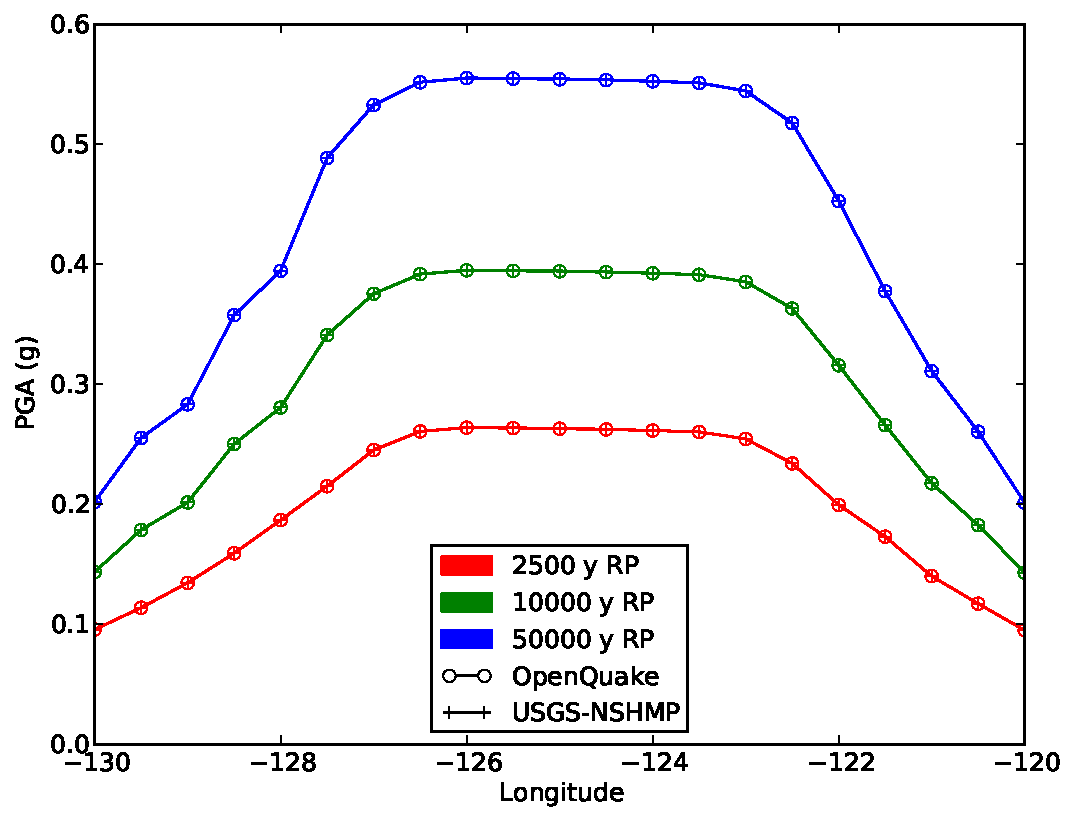
\includegraphics[width=12.5cm]{./qareport/pictures/cascadia_char_oq_nshmp_ew.pdf}
\caption{Hazard map comparison along EW profile for Cascadia characteristic model}
\label{fig:cascadia_char_ew}
\end{figure}
\begin{figure}
\centering
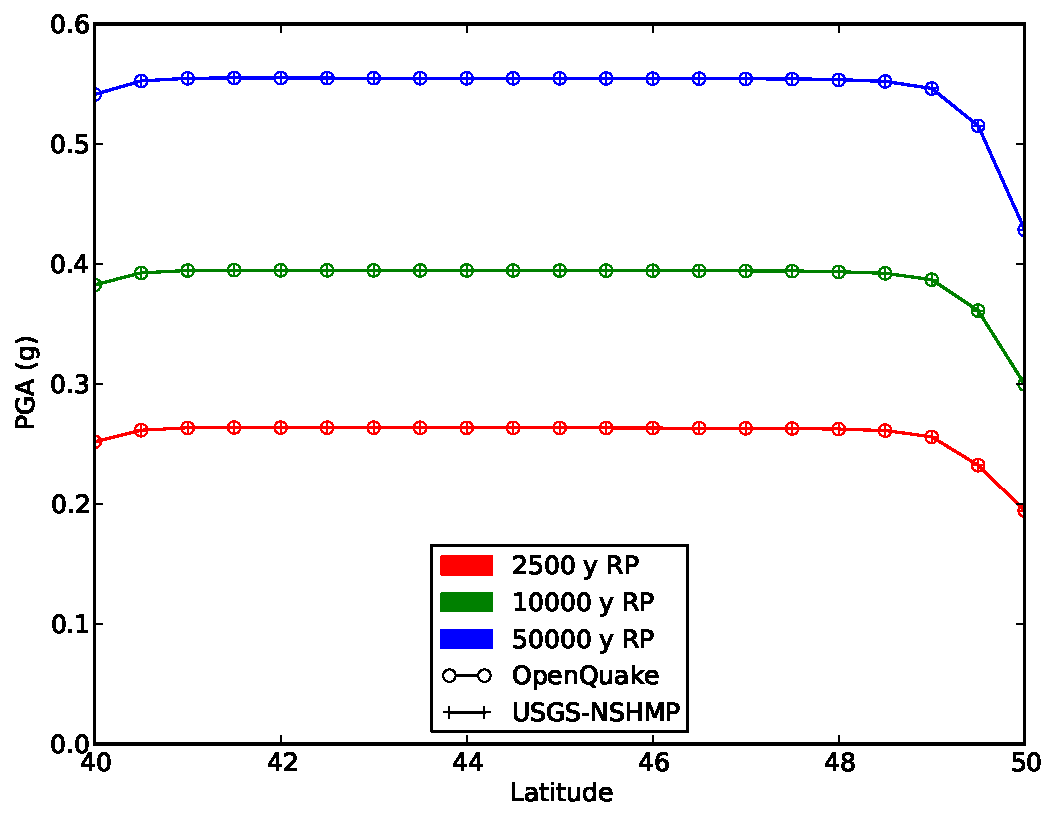
\includegraphics[width=12.5cm]{./qareport/pictures/cascadia_char_oq_nshmp_ns.pdf}
\caption{Hazard map comparison along NS profile for Cascadia characteristic model}
\label{fig:cascadia_char_ns}
\end{figure}

\begin{figure}
\centering
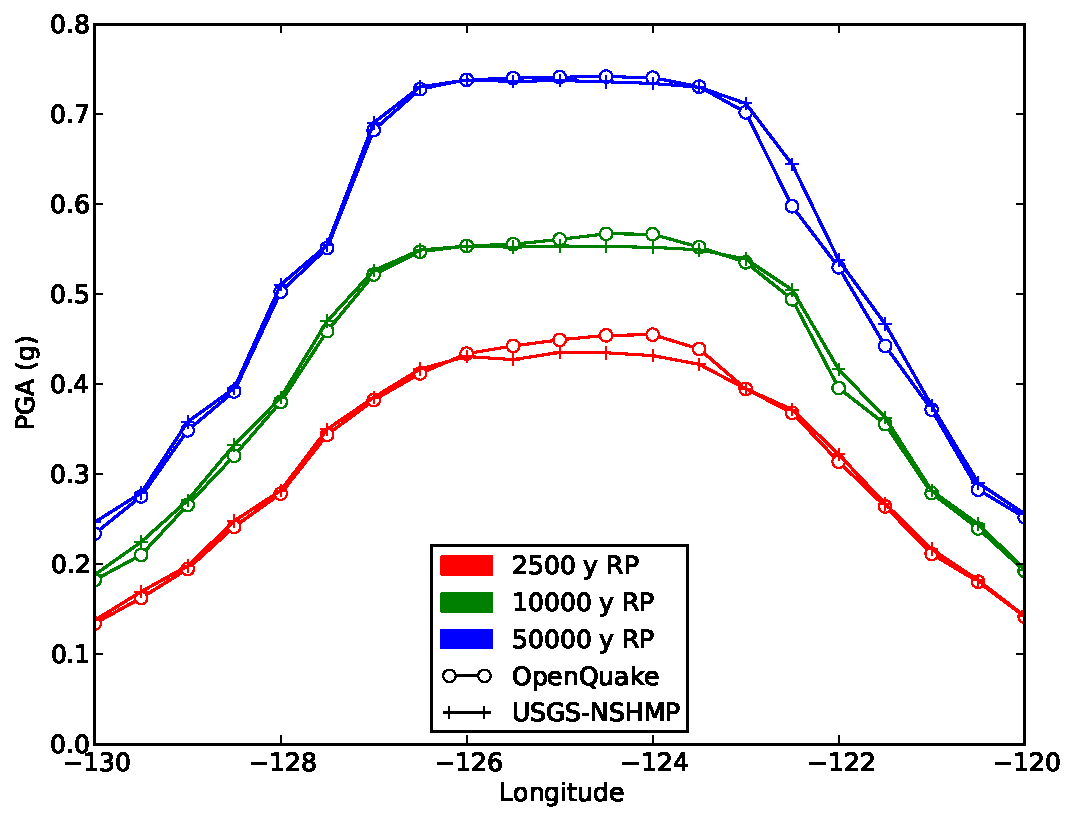
\includegraphics[width=12.5cm]{./qareport/pictures/cascadia_float_oq_nshmp_ew.pdf}
\caption{Hazard map comparison along EW profile for Cascadia unsegmented model}
\label{fig:cascadia_float_ew}
\end{figure}
\begin{figure}
\centering
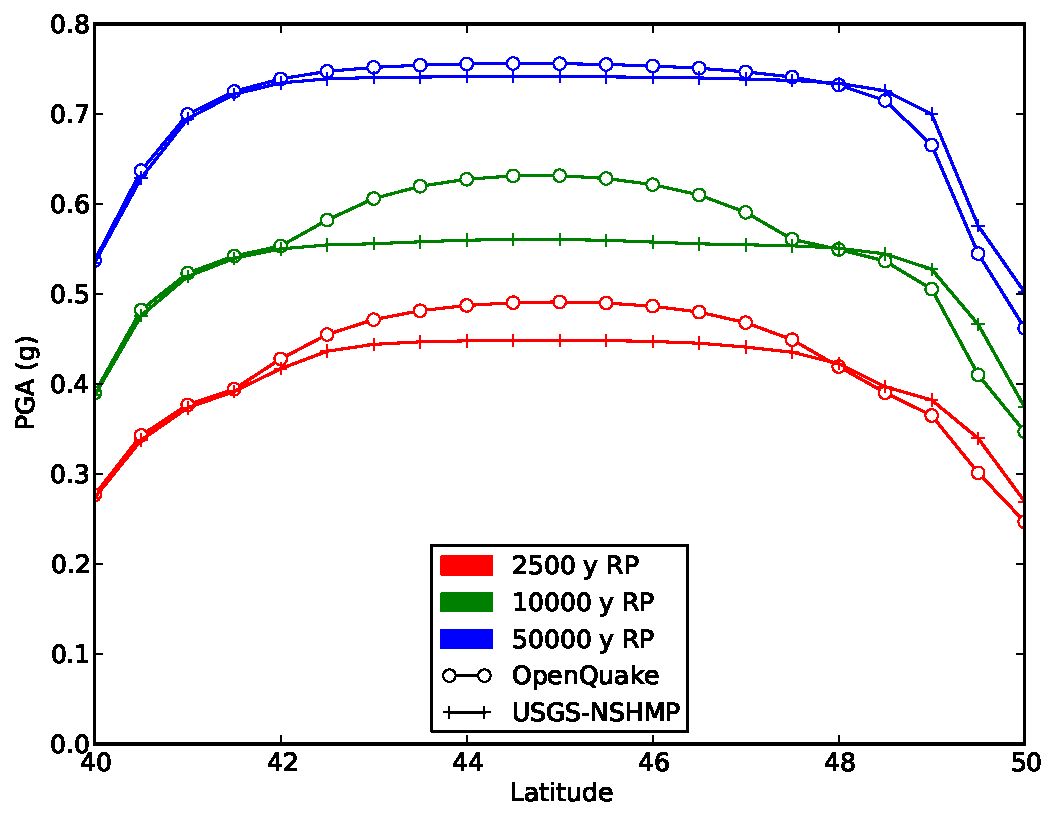
\includegraphics[width=12.5cm]{./qareport/pictures/cascadia_float_oq_nshmp_ns.pdf}
\caption{Hazard map comparison along NS profile for Cascadia unsegmented model}
\label{fig:cascadia_float_ns}
\end{figure}

%----------------------------------------------------------------------------------------
%	CHAPTER 4
%----------------------------------------------------------------------------------------
\chapterimage{chapter_head_1.pdf} % Chapter heading image
\chapter{Other PSHA codes: real cases}
In this chapter we present comparisons between seismic hazard results computed
using OpenQuake-engine and alternative software for real PSHA. We present three
cases: the seismic hazard model for the 2005 national building code of Canada
(\cite{adams2003}, \cite{halchuk2008}), the 2008 U.S. national seismic hazard
model (\cite{petersen2008}), and the seismic hazard model for a nuclear power
plant in South Africa (\cite{bommer2013}). We refer the reader to the original
reports for an in-depth description of each model. Here we present only the
main features and the aspects of interest for the software implementation.
%
% ..............................................................................
\section{The 2005 Canada national seismic hazard model}
%
% ..............................................................................
\subsection{The seismic source model}
To capture epistemic uncertainties in the seismic source definition, two
complete seismic source models are defined in the Canada national seismic hazard
model: the historical (\textbf{H}) and regional (\textbf{R}) models. The
historical model uses relatively small source zones drawn around historical
seismicity clusters, while the regional model defines larger, regional zones
reflecting seismotectonic units. Both models are composed of area sources, with
the only exception of the Queen Charlotte fault (in western Canada) modelled as
a fault source. 

Occurrence rates for each source are defined through a double-truncated
Gutenberg-Richter distribution, with minimum magnitude equal to 4.75. Epistemic
uncertainties in the magnitude-frequency distribution are captured by the
definition for each source of three possible ($a_{GR}$, $b_{GR}$) pairs and
three possible maximum magnitudes. Each source is also associated to three
possible hypocentral depths.

The model prescribes also a floor model (\textbf{F}) for the relatively aseismic
central part of Canada and a deterministic model for the Cascadia subdution zone
(\textbf{C}). Earthquake ruptures associated with area sources are assumed to
have no spatial extension (that is point ruptures), while earthquakes on faults
follow a magnitude-length scaling relationship ($L=10^{-1.085 + 0.389 m}$).
%
% ..............................................................................
\subsection{The ground motion model}
The ground motion model distinguishes between eastern and western Canada because
of the different properties in the crust. For eastern and central Canada the
GMPE model of \citet{ab1995} is used. For western Canada the model of
\citet{bjf1993} is used for shallow crustal sources, while for deep intraslab
sources the model of \citet{y1997} is adopted. Epistemic uncertainties are
included by defining, for each GMPE, a pair of parallel alternative relations,
with higher and lower mean values.
%
% ..............................................................................
\subsection{Reference site conditions}
Hazard maps are computed for a \textit{reference} ground condition corresponding
to "Site Class C" (firm-ground), defined by a 360 to 750 m/s $Vs_{30}$. For
central and eastern Canada, hazard map values computed with the hard-rock GMPE
of \citet{ab1995} are adjusted for firm-ground. That is, seismic hazard spectral
values are amplified by a period-dependent 'reference ground condition' factor
(see Table 2 in \cite{adams2003}). For western Canada, the model of
\citet{y1997} is adjusted for firm-ground. The model of \citet{bjf1993} does not
require instead any adjustment given that its "Soil Class B" is identical to
"Site Class C".
%
% ..............................................................................
\subsection{Implementation of the model in the OpenQuake-engine}
Currently, only the \textbf{H} and \textbf{R} models are implemented in the
OpenQuake-engine. We set the discretization step for area sources to 5 km, and
model ruptures as points. The discretization step for the Queen Charlotte fault
is instead 2 km, and the rupture extension is modeled using the magnitude-area
scaling relationship of \citet{wells1994}. The OpenQuake-engine does not
currently support the inclusion of magnitude-length scaling relationships and
this prevent us from exactly reproducing the original rupture modeling for the
Queen Charlotte fault.

For each source in both the \textbf{H} and \textbf{R} model, we computed a mean
magnitude-frequency distribution by considering all possible (that is 9)
($a_{GR}$, $b_{GR}$) - $M_{max}$ combinations. That is, for each magnitude bin
(of 0.1 magnitude units width), we defined the occurrence rate as the weighted
mean of the rates obtained from the different possible magnitude-frequency
distributions.

For each site, contributions from ruptures that are within a radius of 600 km
are considered for the central and eastern Canada models and of 400 km for the
western Canada models (consistently with what reported by \cite{adams2003}). The
original calculation assumes the ground motion distribution to be untruncated.
To reproduce such condition, we assume in the OpenQuake-engine calculation a
truncation level equal to 6 sigmas.
%
% ..............................................................................
\subsection{Comparison against Canada hazard maps}
We compare the OpenQuake-engine results against hazard maps obtained from
\textit{mean} hazard curves produced by the Geological Survey of Canada (GSC)
using a modified version of the commercial software FRISK88
(http://www.riskeng.com/software/frisk88m/). The GSC approach for constructing
hazard maps (for a given probability of exceedance or return period) relies on
the so-called 'robust' method (\cite{adams2003}). The method is based on
choosing, from the four models (\textbf{H}, \textbf{R}, \textbf{F} and
\textbf{C}), the highest value for each grid point accross Canada.

Using the OpenQuake-engine we thus computed hazard map values for the sites
across Canada for which the \textbf{H} or \textbf{R} models give the highest
values. A comparison for the $10\%$ probability of exceedance map for PGA is
shown in Figure \ref{fig:canada_475y_hmaps}.
\begin{figure}
\centering
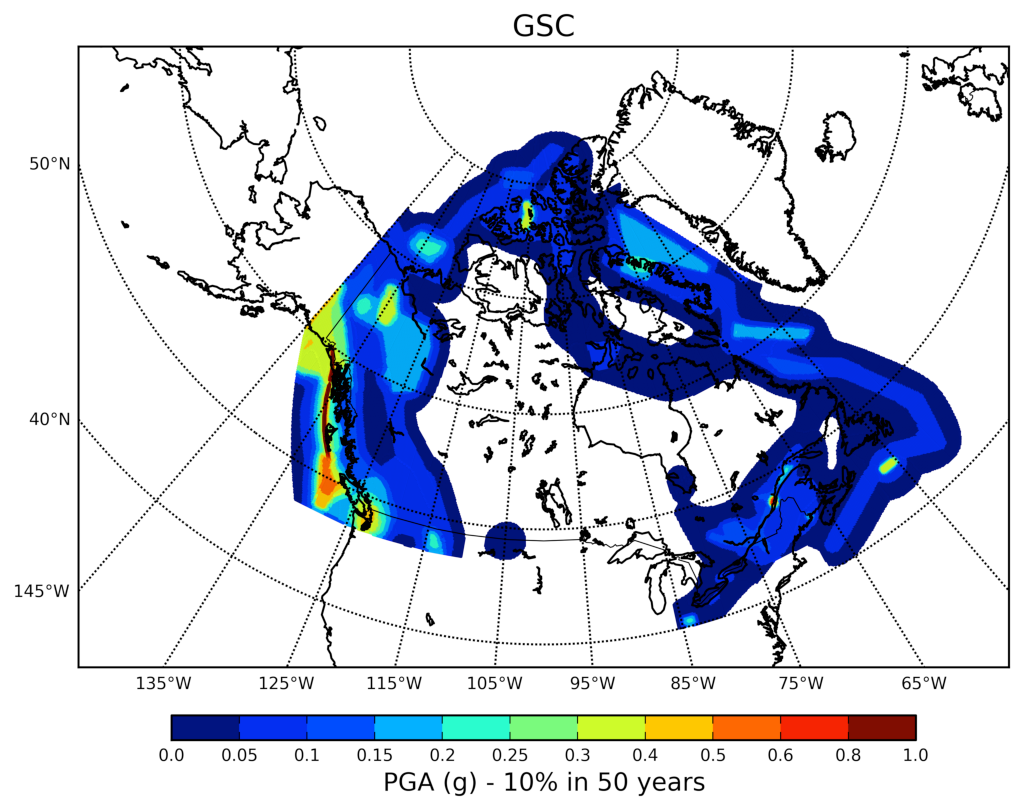
\includegraphics[width=14cm]{./qareport/pictures/GSC_combined_PGA_0pt1_firm_ground.pdf}
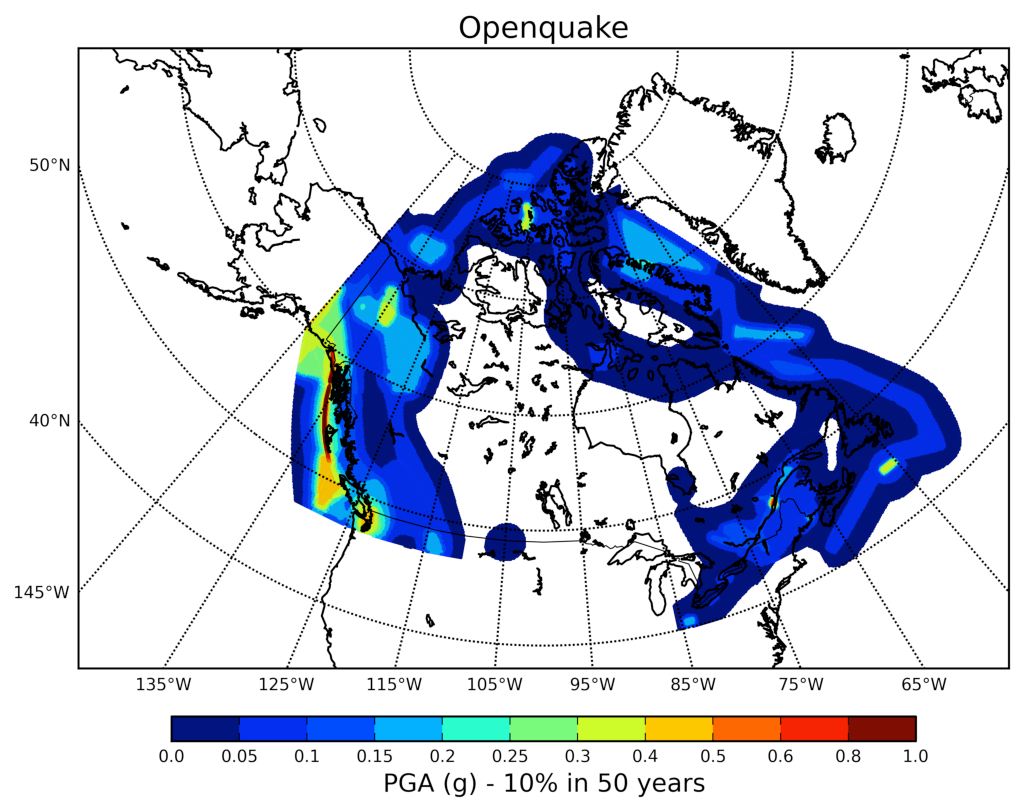
\includegraphics[width=14cm]{./qareport/pictures/OQ_combined_PGA_0pt1_firm_ground.pdf}
\caption{Official hazard map produced by the Geological Survey of Canada (top) and by the OpenQuake-engine implementation (bottom)}
\label{fig:canada_475y_hmaps}
\end{figure}
\begin{figure}
\centering
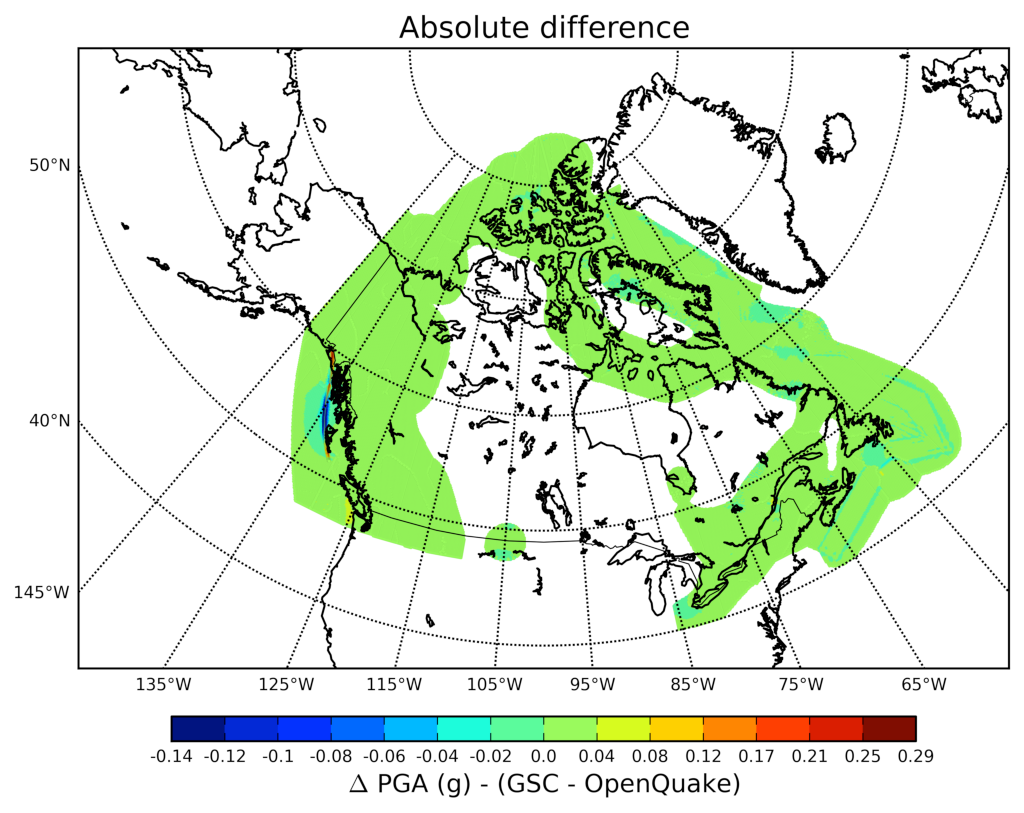
\includegraphics[width=14cm]{./qareport/pictures/GSC_OQ_PGA_0pt1_abs_diff.pdf}
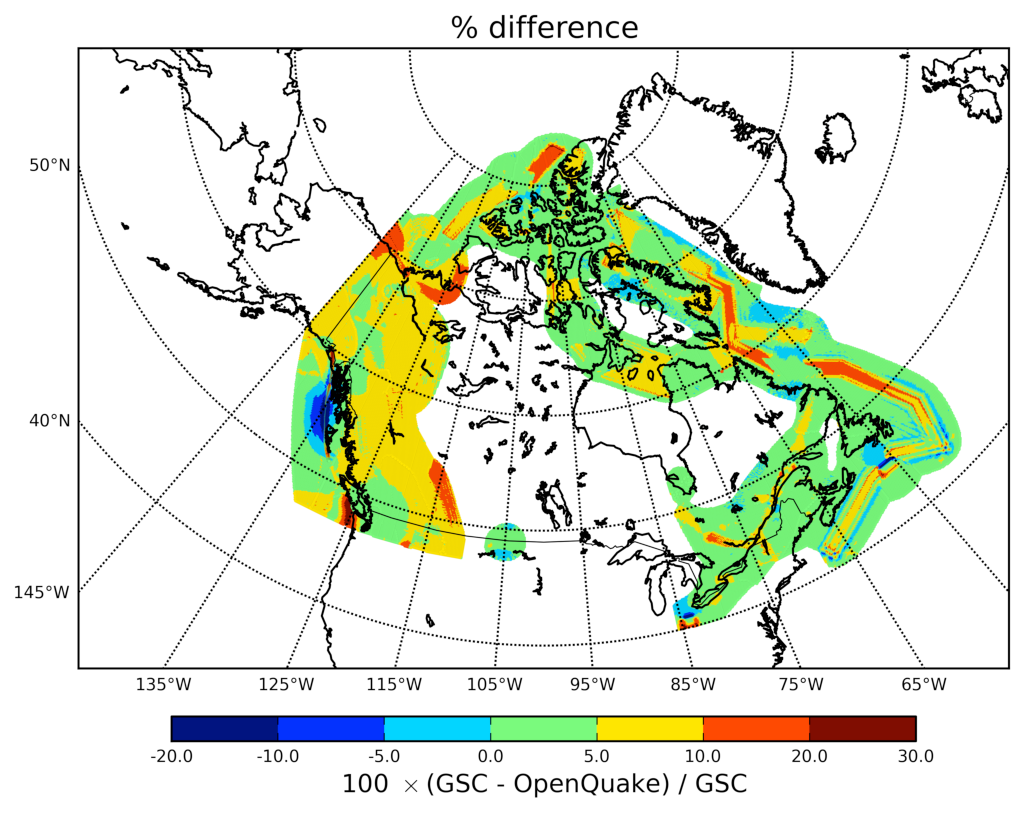
\includegraphics[width=14cm]{./qareport/pictures/GSC_OQ_PGA_0pt1_percent_diff.pdf}
\caption{Absolute (top) and percent (bottom) difference maps between the official GSC hazard map and the one produced by the OpenQuake-engine as visible in Figure \ref{fig:canada_475y_hmaps}}
\label{fig:canada_475y_dmaps}
\end{figure}
The comparison between the hazard maps reveals a satisfactory agreement, at
least from a visual perspective. Difference maps (Figure
\ref{fig:canada_475y_dmaps}) are however more informative and provide a
quantitative understanding of the differences between the two maps.

The absolute difference map shows that for the vast majority of the grid points,
the GSC solution over-estimates the OpenQuake-engine solution by values between
0 and 0.04 g. The highest positive differences (GSC > OpenQuake-engine), up to
0.3 g, are instead only visible along the Queen Charlotte fault, especially at
the north and south endings of the fault trace. The highest negative differences
(GSC < OpenQuake-engine) are still along the Queen Charlotte fault, especially
in the region close to the middle part of the fault trace. These differences can
be reasonably motivated by the previously mentioned fact that, for the Queen
Charlotte fault, we cannot use in the OpenQuake-engine a magnitude-length
scaling relationship as originally defined by the model. We thus used the
\citet{wells1994} magnitude-area scaling relationship. The discrepancies reflect
not only different functional forms but also different ways of defining
ruptures' size and shape. Indeed when using a magnitude-length scaling
relationship, no rupture reshaping (for area conservation) is required which is
instead a key feature when considering a magnitude-area scaling law.

The relative percent error shows instead the significance of the absolute
difference in the various regions covered by the hazard map. Percent differences
ranges from $-20\%$ to $30\%$. The highest positive differences are visible
along the area sources associated with low hazard values. Some significant
differences are visible along the boundaries of rectangular zones such as the
small rectangular area source close to the village of Anna, in Ohio, U.S. (85W,
40N) and the source south of the Newfoundland, Canada (approximately 60W, 45N).
Inside those sources the hazard levels are relatively high (between 0.15 and 0.2
g for the former and between 0.3 and 0.4 for the latter). Within the boundary
the relative error is less than $5\%$. The larger differences along the boundary
may be therefore the effect of different discretization algorithms in the two
software.
%
% ..............................................................................
\section{The 2008 U.S. national seismic hazard model}
%
% ..............................................................................
\subsection{The seismic source model}
To reproduce earthquake occurrences in various tectonic settings, the seismic
source model defines different typologies of seismic sources:
gridded-seismicity, uniform seismicity zones, and fault sources.

Gridded-seismicity and source zones are used to model seismicity occurring off
known faults, and moderate-size earthquakes not included in fault sources.
Occurrence rates are defined through a Gutenberg-Richter magnitude frequency
distribution, with minimum magnitude equal to 5. Earthquakes smaller than $M=6$
are treated as point ruptures, while for larger events finite ruptures are
generated. Rupture lengths are determined by using the magnitude-length scaling
relationship of \citet{wells1994}. Uncertainties in rupture strike are taken
into account by assigning to each site an average distance from ruptures with
strike directions uniformly distributed from $0^{\circ}$ to $180^{\circ}$.
Dipping ruptures are also modeled in the western U.S. by including an average
hanging-wall effect.

For the most part, fault sources are defined to model earthquakes with magnitude
larger than 6.5. Alternative fault source models are defined to take into
account different magnitude-frequency distributions: Characterisitic
\citep{schwartscoppersmith1984} and Gutenberg-Richter. Alternative fault
geometries are also included.

The source model distinguishes between central and eastern U.S. (CEUS) and
western U.S. (WUS). In CEUS the maximum magnitude is distributed between 6.6 and
7.2 for cratonic regions, and between 7.1 and 7.7 for the extended margin. Four
alternative gridded-seismicity models are defined: three that take into account
different completeness levels and one that considers uniform source zones for
the Eastern Tennessee and New Madrid seismic zones. A number of uniform
background zones are also defined to provide a hazard floor in areas with little
or no historical seismicity. Fault sources are defined for the New Madrid
seismic zone, and for the Meers fault (Oklahoma) and Cheraw fault (Colorado).
For New Madrid, five possible fault traces are defined and three possible return
periods (500-year, 750-year, 1000-year) are considered. Moreover, a temporal
clustering model is also included which considers the possible occurrence of
three dependent events. For the Charleston (South Carolina) seismic zone, two
source zones are defined in connection with the $M=7.3$ event occurred in 1886.

In WUS, the maximum magnitude for gridded (shallow) seismicity is 7.0 in most
regions. Exceptions include areas close to modeled faults. If a fault follows a
Gutenberg-Richter magnitude frequency distribution, then the maximum magnitude
in the neighbouring region is set to 6.5 (which is the $M_{min}$ of the fault
Gutenberg-Richter relation). If a fault follows a Characteristic model, then the
maximum magnitude is set to the minimum between 7.0 and the fault characteristic
magnitude. For deep seismicity, the maximum magnitude is instead set to 7.2. For
shallow seismicity, a single gridded-seismicity model is defined which, together
with a number of uniform background zones and special zones, represent the
overall distributed seismicity in WUS. Fault sources are defined for specific
regions: the Intermountain West, Pacific Northwest (including Cascadia
subduction faults), and California. Earthquake occurrence rates are both
described by a Characteristic and Gutenberg-Richter distribution. Epistemic
uncertainties of $\pm 0.2$ magnitude units are defined for both the
Characteristic earthquake magnitude and the maximum magnitude of the
Gutenberg-Richter relation. In addition to epistemic uncertainties, aleatory
variability is included for characteristic earthquakes using a normal
distribution with standard deviation of 0.12.
%
% ..............................................................................
\subsection{The ground motion model}
The ground motion model specifies different sets of GMPEs for CEUS and WUS. For
CEUS, a set of seven GMPEs is defined to represent the epistemic uncertainties
in the ground motion modeling: \citet{frankel1996}, \citet{somerville2001},
\citet{campbell2003SCR}, \citet{toro1997}, \citet{atkinson2006},
\citet{tavakoli2005}, \citet{silva2002}. For active shallow crust in WUS, the
GMPEs used are \citet{boore2008}, \citet{campbell2008}, and \citet{chiou2008}.
For subduction interface events (Cascadia) the GMPE models adopted are:
\citet{y1997}, \citet{ab2003}, \citet{zhao2006}. For subduction intraslab the
GMPEs of \citet{geomatrix1993} and \citet{ab2003} are used instead. For active
shallow crust in WUS, an additional level of epistemic uncertainties is included
to take into account data limitations especially for large earthquakes. Indeed,
for each GMPE, two symmetrical relationships are obtained by adding/subtracting
a scaling factor to the median value.
%
% ..............................................................................
\subsection{Reference site conditions}
Hazard maps are computed for a reference site condition corresponding to the
'NEHRP B/C site' condition which is associated to a $V_{s30}$ value equal to
760.0 m/s. The GMPEs used for active shallow crust in WUS allows for a direct
usage of the $V_{s30}$ value. For subduction GMPEs the 'rock' site class is
selected instead. Some of the CEUS GMPEs do not support the B/C site conditions.
Therefore a 'kappa' correction is applied to convert CEUS GMPEs from hard rock
to firm rock condition.
%
\begin{figure}
\centering
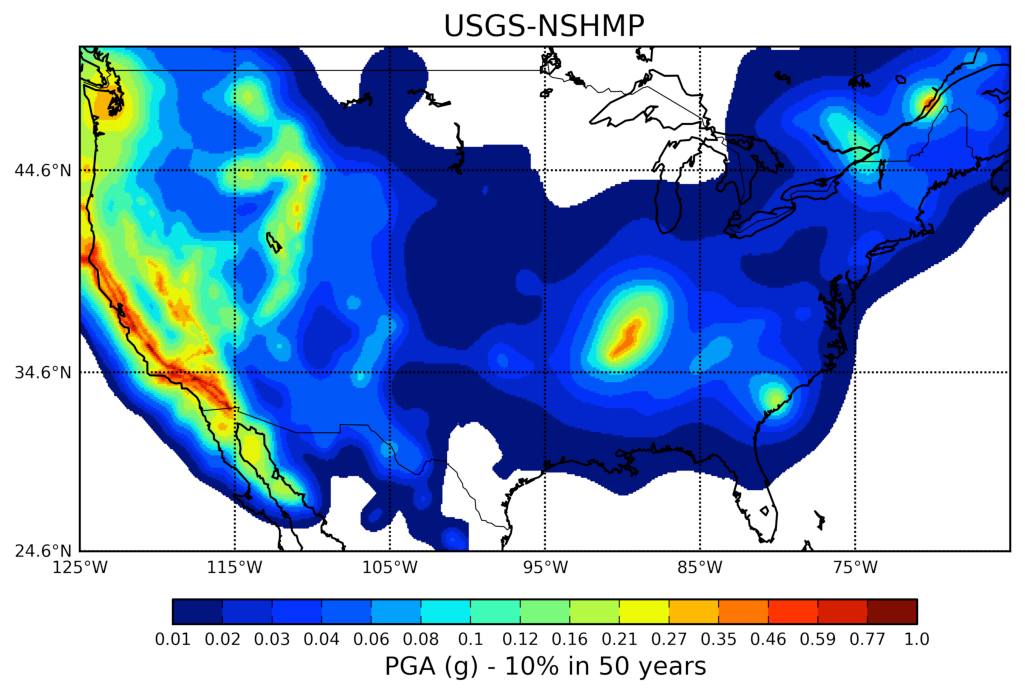
\includegraphics[width=14cm]{./qareport/pictures/map_usa_PGA_0pt1_NSHMP.pdf}
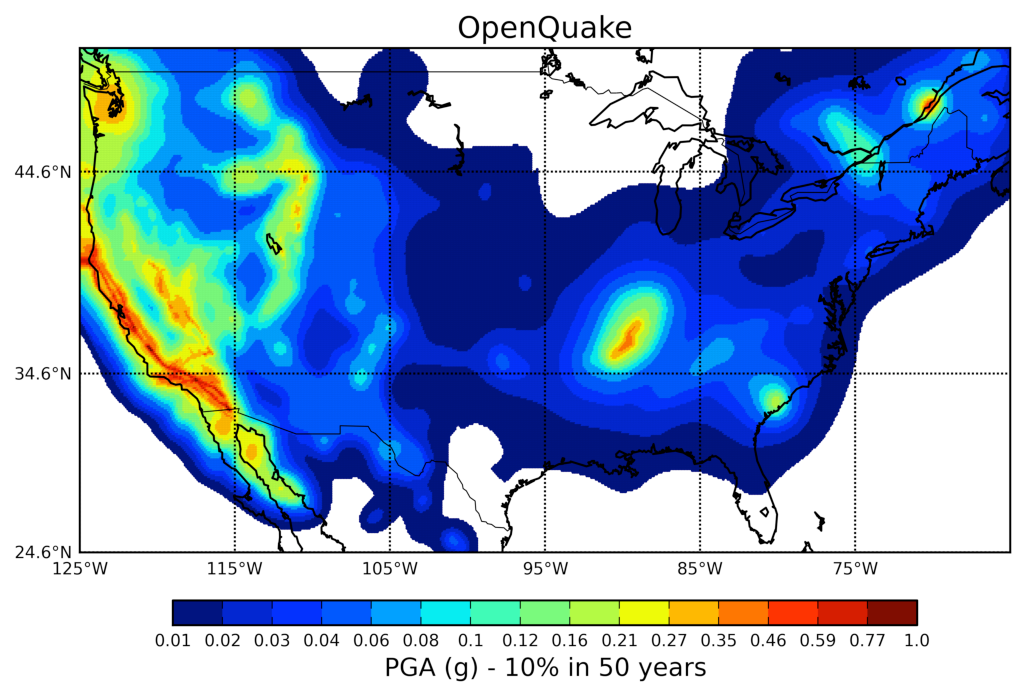
\includegraphics[width=14cm]{./qareport/pictures/map_usa_PGA_0pt1_OQ.pdf}
\caption{Official hazard map produced by the USGS-NSHMP (top) and by the OpenQuake-engine implementation (bottom)}
\label{fig:usa_475y_hmaps}
\end{figure}
\begin{figure}
\centering
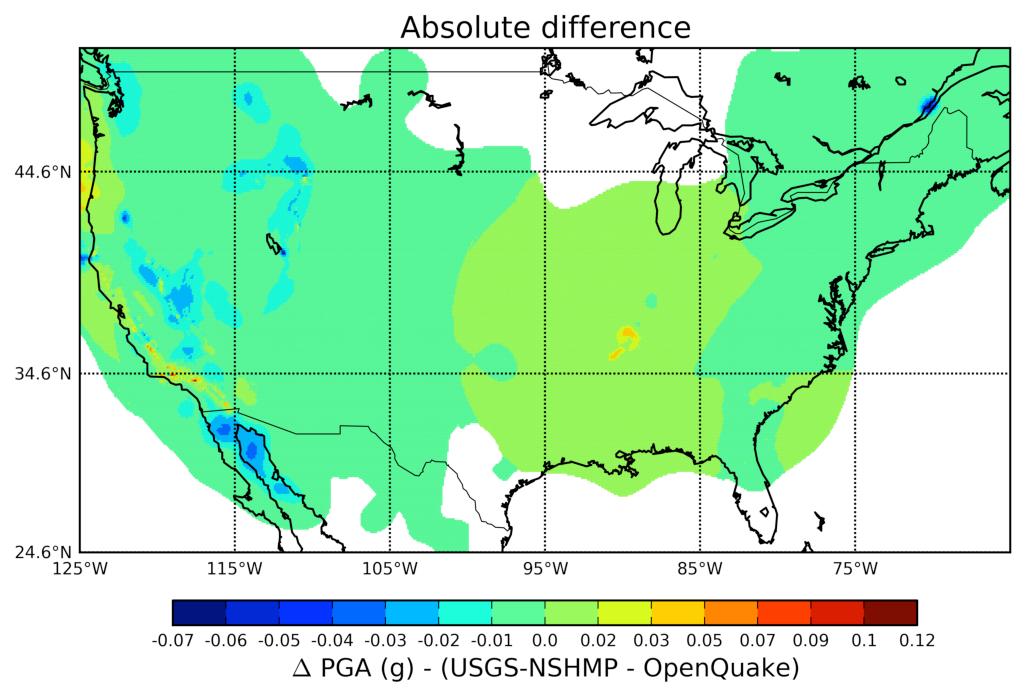
\includegraphics[width=14cm]{./qareport/pictures/map_usa_PGA_0pt1_abs_diff_NSHMP_OQ.pdf}
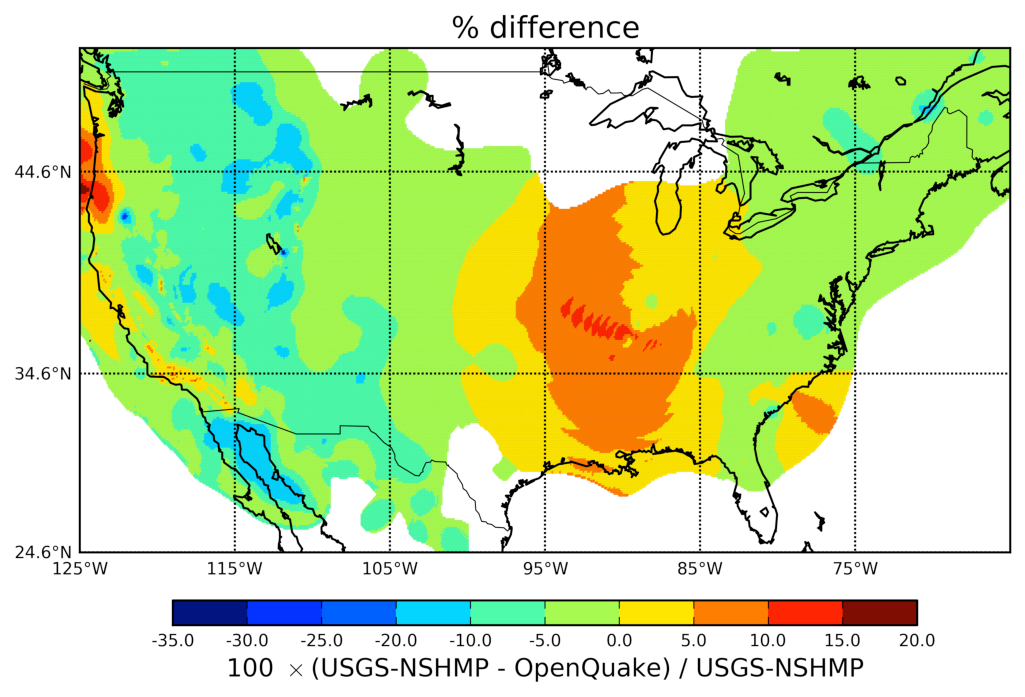
\includegraphics[width=14cm]{./qareport/pictures/map_usa_PGA_0pt1_percent_diff_NSHMP_OQ.pdf}
\caption{Absolute (top) and percent (bottom) difference maps between the
official USGS-NSHMP hazard map and the one produced by the OpenQuake-engine as
visible in Figure \ref{fig:usa_475y_hmaps}}
\label{fig:usa_475y_dmaps}
\end{figure}
%
% ..............................................................................
\subsection{Implementation of the model in the OpenQuake-engine}
In the OpenQuake-engine implementation, gridded-seismicity models and uniform
seismicity zones are defined as collections of point sources. Point source
properties reflect model's specification. If the model defines uncertain
ruptures strike, then each point source is associated to multiple strike values
(between $0^{\circ}$ and $180^{\circ}$ for vertical ruptures and between
$0^{\circ}$ and $360^{\circ}$ for dipping ruptures) otherwise a single strike is
defined. For 'shallow' gridded seismicity models, the hypocentral depth is set
to 7.5 km (equal to the depth of the centroid of dipping rupture planes
(\cite{petersen2008})) and the lower seismogenic depth is set to 15 km. Deep
seismicity is assumed to occur at an hypocentral depth of 50 km, and the
seismogenic layer is assumed to extend between 50 and 100 km. Crustal faults are
defined as simple fault sources (with discretization step of 4 km), while
Cascadia subduction interface faults are defined as complex fault sources (with
discretization stepf of 10 km). The magnitude-area scaling relationship of
\cite{wells1994} is used for all models (gridded-seismicity and fault based)
both in WUS and CEUS. In the current OQ-engine implementation, all source models
are included except the cluster model for the New Madrid seismic zone (only the
unclustered source model is considered). To combine models from different logic
tree branches, we compute for each source a magnitude-frequency distribution
whose occurrence rates are scaled by the branch weight. For each site,
contributions coming from ruptures that are within 1000 km are considered for
the CEUS and Cascadia models, and 200 km for the gridded-seismicity and the
shallow crustal faults models in WUS. Ground motion distribution is truncated at
three sigmas (\cite{petersen2008}). Epistemic uncertainties on GMPE median
values for WUS active shallow crust are not yet implemented.
%
% ..............................................................................
\subsection{Comparison against USA hazard map}
The comparison between PGA hazard maps for $10\%$ probability of exceedance in
50 years produced by the USGS-NSHMP and by the OpenQuake-implementation is shown
in Figure \ref{fig:usa_475y_hmaps}. The visual comparison shows an overall
agreement. A more quantitative view on the differences between the two maps is
given in Figure \ref{fig:usa_475y_dmaps}. Absolute differences range from -0.07
g to 0.12 g. For the vast majority of the sites, differences range from -0.01 g
0.02 g. Close to WUS crustal faults (except California) and in the Charlevoix
(Quebec, Canada) zone the OQ-engine provides larger values. On the contrary,
close to some southern California crustal faults and close to the New Madrid
zone the OQ-engine provides lower values than the USGS-NSHMP. This is also
visible in the percent difference map, where in a broad area around the New
Madrid seismic zone differences range mostly from $0$ to $10\%$ with peak values
up to $15\%$. Lower values in the OpenQuake-engine solutions are also visible
close to the Charleston zone and in Oregon/Washington states (WUS).

Differences in the New Madrid zone can be accounted for by the absence, in the
OQ-engine implementation, of the clustered source model. Discrepancies in the
WUS can be instead explained as due to the missing epistemic uncertainties in
the GMPE median value for shallow crustal sources. In addition to that,
differences can arise because of the different scaling relationship used. In
California, the model of \cite{hanks2002} is used, while in the OpenQuake-engine
calculation the model of \cite{wells1994} is adopted.
%
% ..............................................................................
\section{PSHA for the Thyspunt nuclear site in South Africa}
\citet{bommer2013} describes the use of the OpenQuake-engine for validating
the logic-tree implementation in a PSHA carried out for the coastal site of
Thyspunt, on the southern coast of South Africa, a location selected for the
possible construction of a new nuclear power plant.

The PSHA, done following the guidelines of a SSHAC level 3 project
(\cite{budnitz1997}), required the calculation procedure, and in particular the
implementation of the logic tree representing the full set of uncertainties, to
be subject to Quality Assurance (QA). To provide QA checks, the logic tree was
simultaneously implemented in two different, and entirely independent, software
packages.

The FRISK88 software was selected to perform the official seismic hazard
calculations while the OpenQuake-engine was used as alternative software to
verify the correctness of the logic tree implementation. The seismic source
model consisted of five fault sources and five area sources. 
%
Epistemic uncertainties were defined by considering alternative zone boundaries,
recurrence parameters, fault-ruptures characteristics and maximum magnitude
values. The final logic tree comprised more than 1000 branch combinations for
each area and more than 800 for each fault. 
%
The ground motion model was based on adjusted forms of the GMPEs proposed by 
\citet{abrahamson2008}, \citet{chiou2008}, and \citet{akkar_cagnan_2010} which
in combination of various models for the sigma led to a total of 216 branches in
the ground motion model logic tree.  Considering both the source and ground
motion model logic trees, the number of PSHA input combinations was of the order
of 2 millions.
%
\begin{figure}
\centering
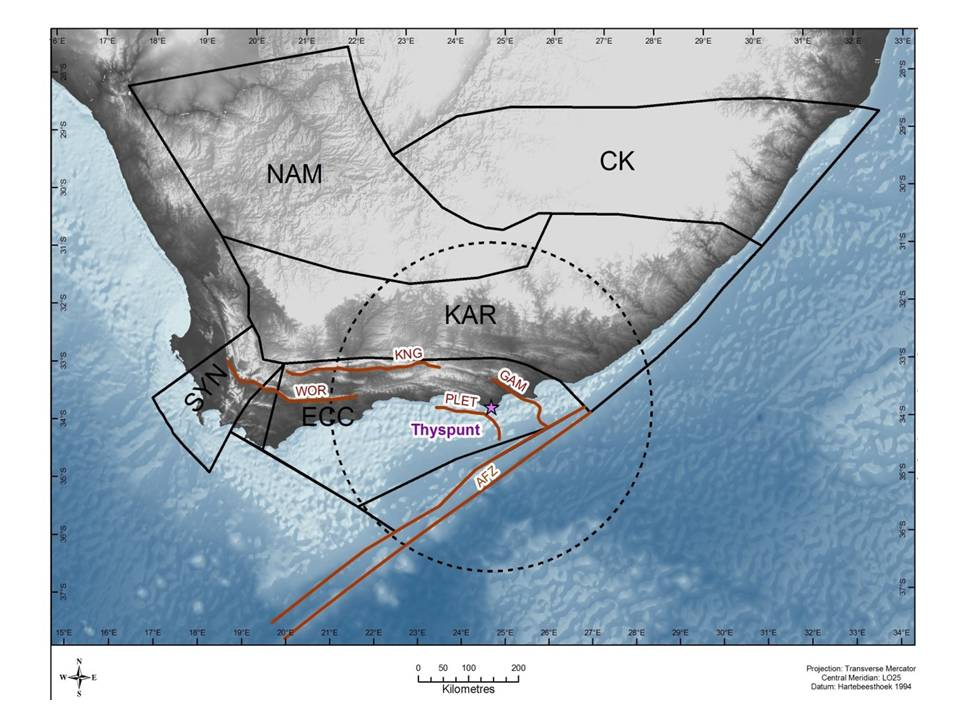
\includegraphics[width=10cm]{./qareport/pictures/ThyspunktSourceModel.jpg}
\caption{Seismic source model (area zones and faults) defined for the Thyspunkt site.}
\label{fig:thyspunkt_source_model}
\end{figure}
%
Verification of the logic tree implementation was carried out by comparing mean
hazard curves for each seismic source considering the full seismic source model
logic tree, but only a single branch in the ground motion model logic tree. In
order to increase the chance of identifying possible errors, all the three GMPE
models were used and three different periods were selected. 
%
Hazard curves computed by the two software for fault and area sources are
presented in Figures \ref{fig:thyspunkt_curves_fault} and
\ref{fig:thyspunkt_curves_area} respectively.

The level of agreement is in general very high considering the complexity in the
seismic source model logic tree. For the two fault sources closest to the site,
PLET and GAM the two pairs of hazard curves are almost identical. For the area
sources, the agreement is generally even better, and neither of the hazard codes
produces consistently higher or lower results.
%
\begin{figure}
\centering
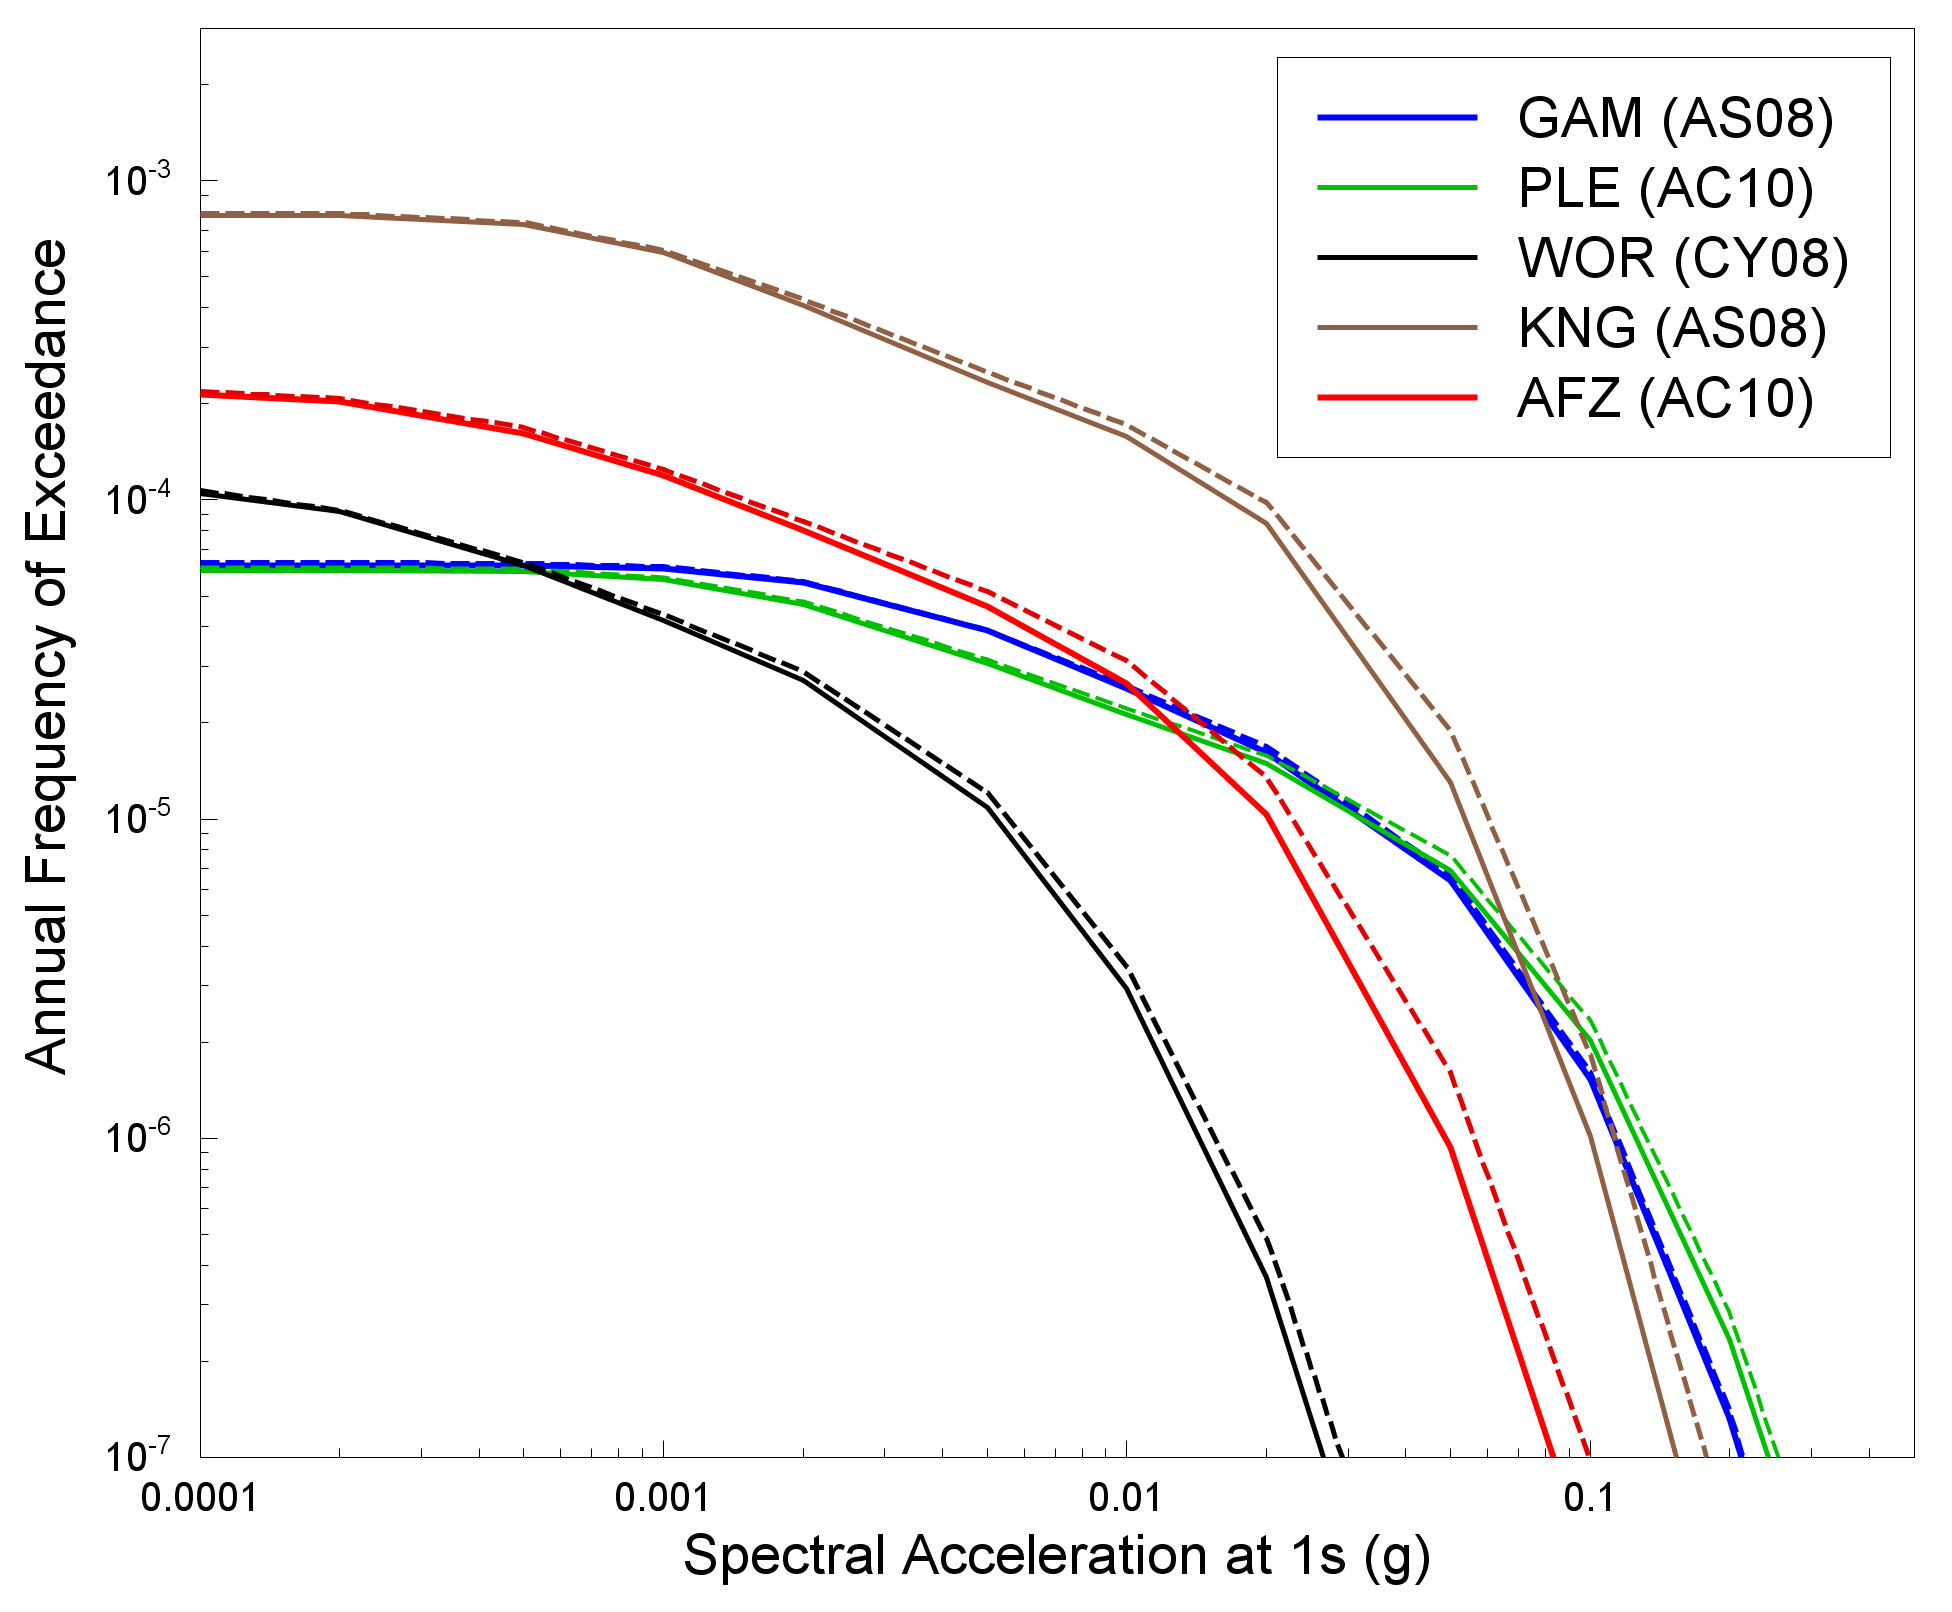
\includegraphics[width=10cm]{./qareport/pictures/ThyspunktCurvesFault.jpg}
\caption{Mean hazard curves obtained for the fault sources using FRISK88 (solid
curves) and the OpenQuake-engine (dashed curves)}
\label{fig:thyspunkt_curves_fault}
\end{figure}
%
\begin{figure}
\centering
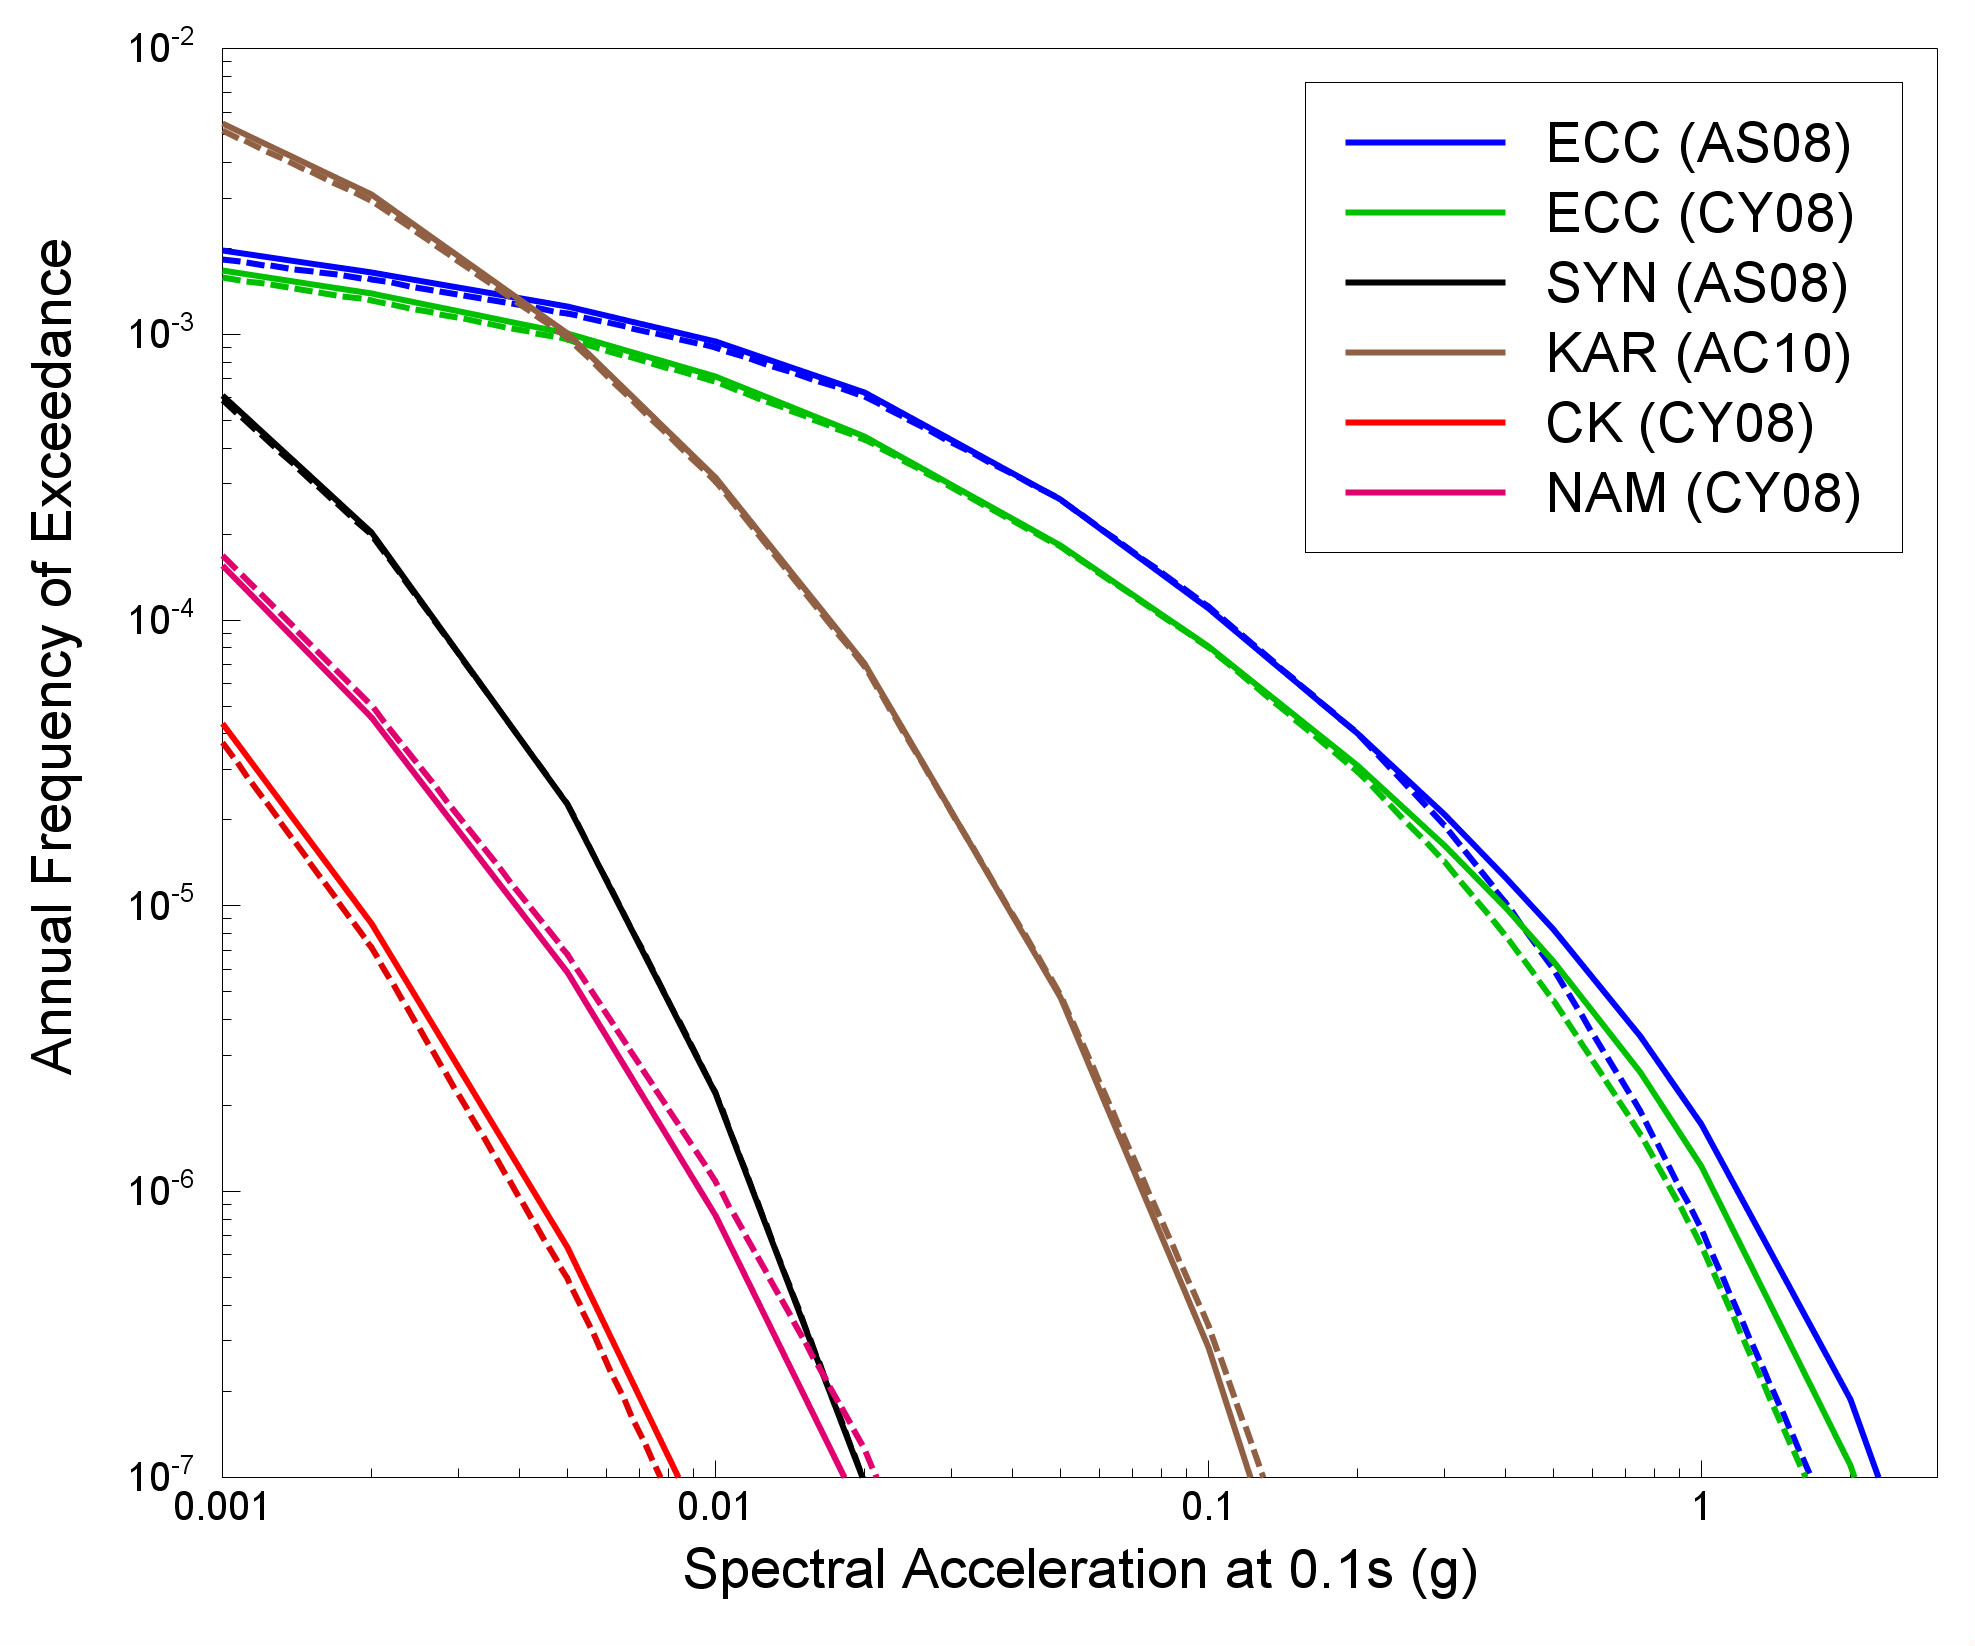
\includegraphics[width=10cm]{./qareport/pictures/ThyspunktCurvesArea.jpg}
\caption{Mean hazard curves obtained for the area sources using FRISK88 (solid curves) and the OpenQuake-engine (dashed curves)}
\label{fig:thyspunkt_curves_area}
\end{figure}

%----------------------------------------------------------------------------------------
%	BIBLIOGRAPHY
%----------------------------------------------------------------------------------------
\chapter*{Bibliography}
\addcontentsline{toc}{chapter}{\textcolor{ocre}{Bibliography}}
\section*{Books}
\addcontentsline{toc}{section}{Books}
\printbibliography[heading=bibempty,type=book]
\section*{Articles}
\addcontentsline{toc}{section}{Articles}
\printbibliography[heading=bibempty,type=article]
\section*{Other Sources}
\addcontentsline{toc}{section}{Reports}
\printbibliography[heading=bibempty,nottype=book,nottype=article]

%----------------------------------------------------------------------------------------
%	INDEX
%----------------------------------------------------------------------------------------
\cleardoublepage
\phantomsection
\setlength{\columnsep}{0.75cm}
\addcontentsline{toc}{chapter}{\textcolor{ocre}{Index}}
\printindex
\printglossary

%----------------------------------------------------------------------------------------

\end{document}
